\documentclass[pdflatex,sn-basic]{sn-jnl}% Basic Springer Nature 
\usepackage{graphicx}%
\usepackage{multirow}%
\usepackage{amsmath,amssymb,amsfonts}%
\usepackage{amsthm}%
\usepackage[title]{appendix}%
\usepackage{booktabs}%
\usepackage{tikz}%
\usetikzlibrary{calc,positioning,arrows.meta}%
\theoremstyle{thmstyleone}%
\newtheorem{theorem}{Theorem}%
\newtheorem{proposition}[theorem]{Proposition}%
\newtheorem{hypothesis}{Hypothesis}%
\newcommand{\wg}{\mathrm{wg}}
\newcommand{\cov}{\mathrm{cov}}
\newcommand{\covgap}{\Delta_{\cov}}
\newcommand{\auroc}{\mathrm{AUROC}}
\newcommand{\Wone}{W_1}
\newcommand{\rhocal}{\rho_{\mathrm{cal}}}
\newcommand{\rhotest}{\rho_{\mathrm{test}}}
\DeclareMathOperator*{\argmax}{arg\,max}
\DeclareMathOperator*{\argmin}{arg\,min}
\raggedbottom
\begin{document}
\title[Worst-Group Conformal Reliability Is More a Calibration Problem]{Worst-Group Conformal Reliability under Spurious Correlation Is More a Calibration Problem than a Representation Problem: A Confound-Controlled Multi-Backbone Study}

\author*[1]{\fnm{One} \sur{Octadion}}\email{octadion@student.ub.ac.id}

\author[1]{\fnm{Novanto} \sur{Yudistira}}\email{yudistira@ub.ac.id}

\author[2]{\fnm{Yuta} \sur{Nakashima}}\email{n-yuta@im.sanken.osaka-u.ac.jp}

\affil*[1]{\orgname{Universitas Brawijaya}, \orgaddress{\city{Malang}, \country{Indonesia}}}

\affil[2]{\orgdiv{SANKEN}, \orgname{The University of Osaka}, \orgaddress{\city{Osaka}, \country{Japan}}}
\abstract{%
Group-robust training methods are certified almost exclusively by worst-group
\emph{accuracy}, while a parallel line of conformal-prediction theory shows that
post-hoc calibration can only \emph{relocate}, never remove, cross-group
heterogeneity in conformity scores. This invites a natural but untested
intuition: that representations made robust on the accuracy side should
\emph{also} carry the conformal (coverage and set-size) reliability of the worst
group. We test that intuition on \emph{both} levers. With the representation held
fixed we run a confound-controlled grid over two benchmarks (Waterbirds, CelebA),
\emph{four} frozen backbones spanning two architecture families and three
pretraining regimes (an ERM-trained ResNet-50, CLIP ViT-B/32, DINOv2 ViT-B/14 and
a supervised ViT-B/16), five last-layer training interventions (ERM, DFR, AFR,
balanced subsampling, last-layer GroupDRO), three nonconformity scores (APS,
RAPS, THR), three calibration policies (marginal split, Mondrian
group-conditional, shift-robust), and a calibration-to-test correlation-strength
sweep; separately, we move the representation \emph{itself}, fine-tuning the
backbone end-to-end under ERM, GroupDRO and reweighting.
Our central result is a dissociation that holds in every cell of both studies.
Worst-group coverage is governed far more by the calibration mechanism than by
the representation: under marginal calibration it swings by up to $0.358$ across
training methods (ERM collapses to $0.51$), whereas under Mondrian calibration
the cross-training spread never exceeds $0.024$ in any of the eight
backbone--dataset cells, and the \emph{same} ERM model is lifted from
$0.51$--$0.82$ to $0.85$--$0.89$ purely by changing the calibration policy.
Fine-tuning the representation does not overturn this: with the head held fixed,
calibration dominates in all six dataset--score cells. The sub-target level is a
selection effect rather than a validity failure---Mondrian's mean-over-groups
coverage is $0.9024$ against a nominal $0.900$, and the reported statistic is a
minimum over four noisy per-group coverages. Training buys \emph{efficiency}
rather than coverage, but conditional on Mondrian and as a tendency rather than a
law: worst-group set size falls as base accuracy rises, yet with cluster-bootstrap
confidence intervals the per-cell accuracy--size correlation is uninformative in
five of eight cells, so we report a direction rather than an estimate. Robust
training's apparent reduction of cross-group conformity-score divergence is
largely an accuracy effect that, once matched, is modest or unmeasurable, and the
accuracy-best training method is almost always the burden-best. Under the
correlation-strength sweep---which shifts the group mixture rather than the
within-group distribution---Mondrian's worst-group coverage is flat to within
$0.010$. Finally, the spurious attribute remains almost perfectly recoverable
from the deployed representation ($\auroc\in[0.945,0.999]$), so group-conditional
calibration is deployable with \emph{predicted} groups: the gap to the
ground-truth oracle is within $0.02$ in $30$ of $34$ arms, needing no observed
group labels at test time. The practical message is corrective and actionable:
report conformal-burden comparisons at matched accuracy (uncontrolled comparisons
overstate the training-side benefit by an order of magnitude), and reach for
group-conditional calibration---which delivers worst-group coverage from
ordinary, fully auditable representations---before reaching for a more robust
representation.
}
\keywords{conformal prediction, spurious correlation, group robustness, worst-group coverage, group-conditional calibration}
\maketitle

\section{Introduction}
\label{sec:intro}

Conformal prediction \citep{vovk2005,angelopoulos2020,romano2020} turns a point
predictor into set-valued predictions with a distribution-free marginal coverage
guarantee under exchangeability. Under a \emph{spurious correlation}---a
background, demographic, or context feature that co-varies with the label in
training but not at deployment---marginal guarantees mask severe \emph{worst-group}
unreliability: the minority group whose spurious feature is mismatched is
systematically under-covered or receives uninformatively large sets
\citep{cresswell2024}. Two largely separate programs respond. The first improves
\emph{training} so the worst group is accurate: GroupDRO \citep{sagawa2020}, Deep
Feature Reweighting (DFR) \citep{kirichenko2023}, AFR (automatic feature reweighting) \citep{qiu2023}, JTT
\citep{liu2021jtt}, CNC \citep{zhang2022cnc}, evaluated almost entirely on
worst-group accuracy and calibration error \citep{yang2023change}. The second
improves \emph{calibration}: Mondrian and group-conditional conformal prediction
\citep{vovk2005,jung2023,gibbs2023}, Kandinsky calibration for overlapping and
fractional groups \citep{deng2025kandinsky}, multi-distribution robust conformal
prediction \citep{mdcp2026}, adaptive fairness-aware conformal prediction
\citep{afcp2024}. A recent impossibility result formalizes the link: the
calibration policy determines only \emph{whether} cross-group score heterogeneity
surfaces as coverage disparity or as set-size disparity, never whether it appears
at all \citep{burden2026}.

These two programs meet at a widespread but rarely tested intuition: if the worst
group can be made \emph{accurate} by changing the representation, perhaps the same
change makes it \emph{conformally reliable}, so robust training should pay off for
downstream uncertainty quantification. A confound-controlled grid instead returns a
clean \emph{dissociation} (Figure~\ref{fig:c1})---the more useful result for a literature that tends to
credit training-side robustness with conformal benefits it does not separately
provide.

Our contributions are:
\begin{enumerate}
\item \textbf{Coverage is governed far more by calibration than by the backbone
(Section~\ref{sec:c1}).} Holding the model fixed and varying only the calibration
policy, worst-group coverage spreads by up to $0.358$ across training methods under
marginal calibration but by at most $0.024$ under Mondrian, in \emph{every} one of
eight dataset$\times$backbone cells; the same ERM model is lifted by $+0.06$ to
$+0.35$ by the switch alone. Four backbones span two architecture families and three
pretraining regimes, and the two we add behave exactly like the two we first reported.

\item \textbf{The dissociation survives moving the representation itself
(Section~\ref{sec:repr}).} Fine-tuning the backbone end-to-end under ERM, GroupDRO and
reweighting raises worst-group accuracy by up to $+0.222$---the largest gain any
intervention here produces---yet under Mondrian the three resulting representations
deliver worst-group coverage within $0.004$ of one another, while under marginal
calibration they span $0.249$. So this is not an artefact of frozen features.

\item \textbf{Training buys efficiency, not coverage---conditional on Mondrian
(Section~\ref{sec:c2}).} With coverage matched, the most accurate arm yields the
smallest worst-group sets in seven of eight cells. We report this as a direction, not
an estimate: the per-cell accuracy--size correlation rests on three to five methods,
and with a cluster bootstrap five of eight intervals are uninformative.

\item \textbf{A confound-controlled protocol, and how little survives it
(Section~\ref{sec:h1}).} Comparing divergence at matched \emph{model-level} accuracy
leaves exactly one of eight cells with overlapping support, because robust training
moves base accuracy off ERM's operating point and ERM's own accuracy has no seed
variance. Where the comparison is defined, the reduction is real
($\Delta_{\mathrm{APS}}=+0.084\,[+0.076,+0.095]$); elsewhere it is undefined, and
uncontrolled comparisons of divergence conflate two effects.

\item \textbf{Accuracy is a good proxy for conformal burden
(Section~\ref{sec:h2}).} The accuracy-best and burden-best arms differ in five of
eight cells by point estimate, but the difference clears its cluster-bootstrap
interval in only one, and by $0.014$ of coverage.

\item \textbf{Sub-target by selection, and deployable without group labels
(Sections~\ref{sec:h3}--\ref{sec:predgroup}).} Mondrian's mean-over-groups coverage is
$0.9024$ against a nominal $0.900$, so the $0.85$--$0.89$ \emph{minimum} we report is
a min-over-groups selection effect rather than under-coverage; it is flat to within
$0.010$ across the correlation-strength sweep. The spurious attribute stays recoverable
from the deployed representation ($\auroc\in[0.945,0.999]$), so coverage and group
auditing coexist, and group-conditional calibration works with probe-predicted
groups---within $0.02$ of the ground-truth oracle in $30$ of $34$ arms.
\end{enumerate}

The unifying thesis (Section~\ref{sec:discussion}) is that, under spurious correlation,
worst-group conformal reliability is governed by the calibration \emph{mechanism} far
more than by the representation the scores come from---not that the representation is
irrelevant, but that changing it, even by retraining it, buys much less worst-group
coverage than changing how the scores are calibrated. We frame the paper as a
characterization rather than a method. Figure~\ref{fig:overview} states the confound,
the mechanism behind the calibration effect, and the design in one place.

\begin{figure}[t]
\centering
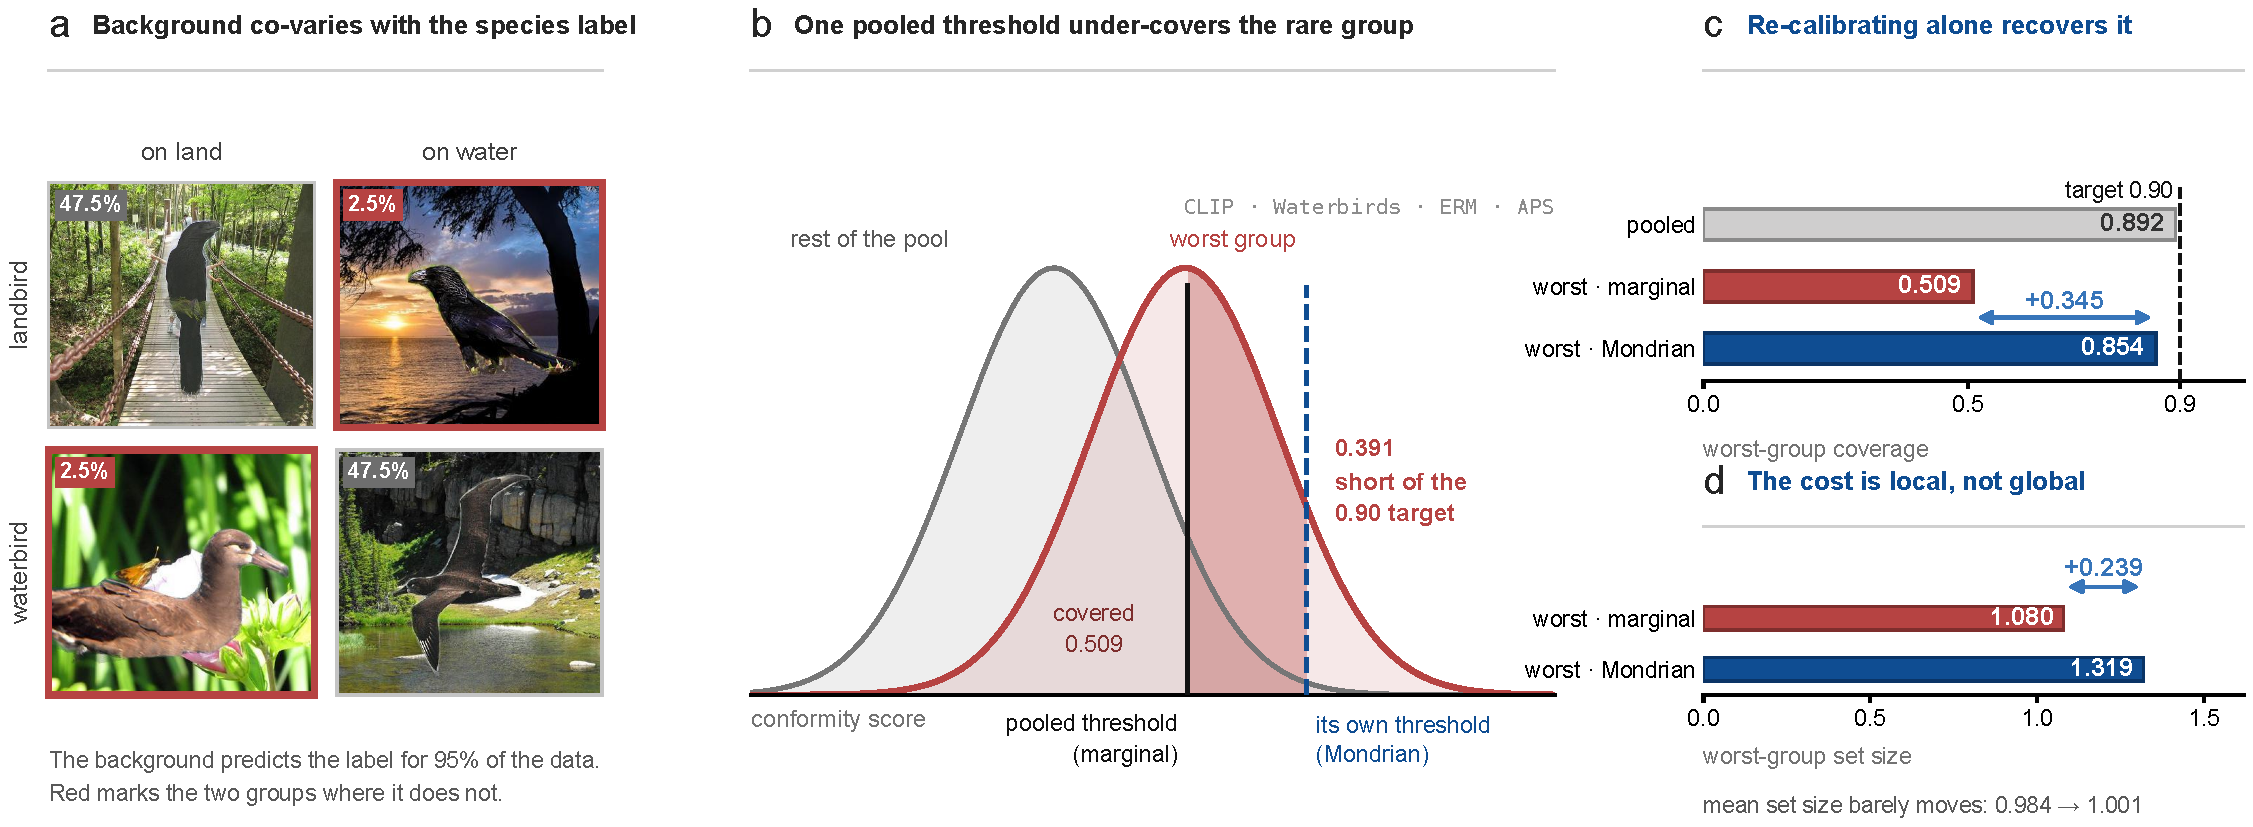
\includegraphics[width=\textwidth]{figures/teaser_method}
\caption{Worst-group conformal reliability is set by the calibration rule, not by the
representation. \textbf{(a)} The confound, on real Waterbirds images, laid out as the
$2\times2$ that defines the groups: species by background. The background predicts the
label for $95\%$ of the data; the two groups where it does not (red) hold $2.5\%$ of the
calibration pool each. \textbf{(b)} Why a single pooled threshold under-covers them. The
curves are the conformity-score distributions of the worst group and of the rest of the
pool, fitted so that the pooled $90\%$ quantile reproduces this cell's measured marginal
worst-group coverage of $0.509$. The shaded wedge, bounded by the pooled threshold and
the group's own, is the shortfall \emph{from the $0.90$ target} given by
Eq.~\eqref{eq:shortfall} in Proposition~\ref{prop:dissociation}(ii). \textbf{(c)} What
that costs, measured. Pooled coverage looks healthy at $0.892$ while the worst group
sits at $0.509$; giving that group its own threshold lifts it to $0.854$ with the model
and its scores untouched. The realised lift of $+0.345$ falls short of (b)'s $0.391$
because Mondrian itself lands below the nominal level, which is the min-over-groups
selection effect of Appendix~\ref{app:subtarget} rather than under-coverage.
\textbf{(d)} What the fix costs in return, and the reason we call the burden moved
rather than removed: the worst group's sets grow from $1.080$ to $1.319$, while the mean
set size moves only $0.984$ to $1.001$. The price of group-conditional coverage is paid
locally, by the group that was previously under-served, and is close to free in
aggregate. Panels (b)--(d) are the CLIP/Waterbirds ERM cell under APS at
$\rhocal=\rhotest=0.95$, averaged over $3$ training seeds $\times$ $10$ calibration
splits; Table~\ref{tab:c1} and Figure~\ref{fig:c1} show the same effect in all eight
backbone--dataset cells.}
\label{fig:overview}
\end{figure}

\section{Related Work}
\label{sec:related}

\paragraph{Group-robust training.} Worst-group accuracy is improved by
distributionally robust optimization \citep{sagawa2020}, last-layer retraining on
group-balanced data (DFR) \citep{kirichenko2023}, automatic feature reweighting
(AFR) \citep{qiu2023}, and pseudo-group methods such as JTT \citep{liu2021jtt} and
CNC \citep{zhang2022cnc}. The standard subpopulation-shift benchmark
\citep{yang2023change} compares these on accuracy-family metrics and calibration
error but reports no set-valued or coverage quantities. Our last-layer arms are
drawn from this zoo so that our worst-group accuracies are comparable to published
values; our object of study is what these interventions do to the \emph{conformal}
side, which this literature does not measure.

\paragraph{Group-conditional and fair conformal prediction.} Mondrian conformal
prediction \citep{vovk2005} computes group-conditional thresholds; conditional
guarantees beyond disjoint groups are given by \citet{gibbs2023} and
\citet{jung2023}, and \citet{deng2025kandinsky} extend group-conditional coverage
to overlapping and fractional memberships. On fairness, \citet{cresswell2024} show
that equalizing coverage can increase disparate impact and recommend equalizing
set sizes; \citet{afcp2024} adaptively equalize coverage while controlling
efficiency; and \citet{burden2026} prove that equalized coverage and equalized set
size cannot in general hold simultaneously, recasting the calibration policy as a
choice of \emph{where} cross-group heterogeneity manifests. Our work is the
empirical complement on the axis these papers hold fixed: we vary the
\emph{training} intervention (hence representation and score distribution) and ask
whether the conserved heterogeneity shrinks at the source. It does not; the
calibration policy remains decisive.

\paragraph{Conformal prediction under shift and for robust models.}
\citet{tibshirani2019} establish validity under covariate shift via likelihood
reweighting; multi-distribution robust conformal prediction \citep{mdcp2026}
targets uniform worst-case coverage as a group-DRO analogue \emph{inside the
calibration procedure}, holding the model fixed---consistent with our finding that
the calibration mechanism is the operative lever. No prior work crosses the
training-intervention zoo with calibration policies under a correlation-strength
sweep, nor controls for the accuracy confound we isolate.

\paragraph{Uncertainty, concepts, and the opposite direction.} Some recent work
uses uncertainty to \emph{improve} group robustness---e.g.\ evidential alignment
that mitigates spurious bias without group labels \citep{evidential2025}---the
reverse of our direction. We treat conformal prediction over learned concept or
concept-bottleneck spaces \citep{conceptconf2025,ncb2024,ncv2025} as an
interpretability layer, orthogonal to our thesis. Selective classification under
group shift \citep{jones2021} found abstention can leave worst-group accuracy flat;
our set-valued analyses extend this lineage to conformal prediction.

\paragraph{Group recovery, conditional coverage, and its limits.} Whether the
protected group can be recovered is a separate question: biased ERM representations
encode the spurious attribute strongly (the principle behind JTT and CNC), which
our probe confirms ($\auroc\in[0.945,0.999]$). This connects to conformal prediction
under noisy class or group labels \citep{einbinder2022,sesia2023noisy}, which
corrects coverage but assumes the group is given; here the group is not noisy but
\emph{recoverable}, which removes the auditability barrier and, via predicted
groups, the deployment barrier (Section~\ref{sec:predgroup}). Finally, exact
feature-conditional coverage is
impossible distribution-free in finite samples \citep{barber2021limits}, which is
why group-\emph{conditional} (Mondrian) coverage is the operative target; online
and multivalid variants \citep{gibbs2023,jung2023} tighten it, but our contribution
holds the calibration family fixed and varies the training intervention---on the last
layer and on the representation itself---to measure how little the representation
substitutes for the mechanism.

\section{Problem Setup and Notation}
\label{sec:setup}

We observe triples $(x,y,a)$ with image $x$, label $y\in\mathcal{Y}$, and binary
spurious attribute $a\in\{0,1\}$ (background/\emph{place} for Waterbirds;
\emph{Male} for CelebA). Groups are $g=(y,a)\in\mathcal{G}$,
$|\mathcal{G}|=2|\mathcal{Y}|$. A frozen backbone $\phi$ maps $x$ to features
$\phi(x)\in\mathbb{R}^d$; a last-layer head $f_\theta$ trained by intervention $m$
maps $\phi(x)$ to class scores. The \emph{correlation strength} $\rho$ is the
evaluation probability that $a$ aligns with $y$ in the majority pattern; we
calibrate at $\rhocal=0.95$ and evaluate over
$\rhotest\in\{0.95,0.9,0.8,0.7,0.6,0.5\}$, holding the calibration distribution
fixed.

\paragraph{Conformal sets and calibration policies.} Given a nonconformity score
$s(x,y)$ and a calibration set $\mathcal{D}_{\mathrm{cal}}$, split conformal
prediction computes
$\hat q=\mathrm{Quantile}_{1-\alpha}\big(\{s(x_i,y_i)\}_{i\in\mathcal{D}_{\mathrm{cal}}}\big)$
and returns $C(x)=\{y\in\mathcal{Y}: s(x,y)\le\hat q\}$. We use three scores: THR
($s_{\mathrm{THR}}(x,y)=1-\hat p(y\mid x)$); APS \citep{romano2020}, the cumulative
softmax mass up to $y$; and RAPS \citep{angelopoulos2020}, APS with a tail
regularizer. We compare three \emph{calibration policies}: \textbf{marginal split}
(one global $\hat q$); \textbf{Mondrian} (a separate $\hat q_g$ per group); and
\textbf{shift-robust} (a reweighted/worst-case threshold over a total-variation ball around the
calibration distribution; Appendix~\ref{app:supp}). Target $1-\alpha=0.90$
throughout; the full configuration is in Appendix~\ref{app:hyper}.

\paragraph{Reliability quantities.} For group $g$, $\cov_g=\Pr[y\in C(x)\mid g]$
and $|C|_g$ is its mean set size. We report worst-group coverage $\min_g\cov_g$
and the \emph{coverage gap}, i.e.\ the worst group's shortfall from the target,
\begin{equation}
\covgap=(1-\alpha)-\min_g\cov_g,
\qquad
\covgap>0 \Leftrightarrow \text{the worst group is under-covered,}
\label{eq:covgap}
\end{equation}
which is the quantity tabulated throughout as the conformal ``burden''. We
distinguish it from the \emph{coverage range} $\max_g\cov_g-\min_g\cov_g$, which
measures dispersion across groups rather than distance from the target and which
we report only where noted. We also report mean set size, the set-size disparity
$\max_g|C|_g-\min_g|C|_g$, and---because $\min_g$ over a finite number of groups is
a downward-biased statistic (Section~\ref{sec:h3})---the unweighted mean over
groups $|\mathcal{G}|^{-1}\sum_g\cov_g$, which is the level group-conditional
calibration actually targets.

\paragraph{Cross-group conformity-score divergence (the ``burden'').} Following the
conserved-quantity view of \citet{burden2026}, we summarize cross-group score
heterogeneity by the divergence between the worst group's conformity-score
distribution $P_{\wg}$ and that of the remaining groups $P_{\neg\wg}$,
\begin{equation}
D=\Wone(P_{\wg},P_{\neg\wg})\quad\text{(Wasserstein-1)},\qquad
D_{\mathrm{KS}}=\sup_t\big|F_{\wg}(t)-F_{\neg\wg}(t)\big|,
\label{eq:div}
\end{equation}
computed per score on a held-out split; $D$ is reported per score (scales differ).

\paragraph{A dissociation principle.} The empirical study is organized around the
following elementary fact, which separates the by-design content of
group-conditional calibration from the substantive question we test.

\begin{proposition}[Calibration--representation dissociation]
\label{prop:dissociation}
Fix a score $s$ and target $1-\alpha$, and assume within-group exchangeability of
calibration and test scores.
\emph{(i)} Group-conditional (Mondrian) split conformal, with per-group threshold
$\hat q_g$ the $\lceil(1-\alpha)(n_g+1)\rceil$-th smallest calibration score in
group $g$, satisfies $\Pr\!\big(Y\in C(X)\mid G=g\big)\ge 1-\alpha$ for every group
$g$, with no dependence on $s$ beyond exchangeability.
\emph{(ii)} Let the scores be continuous, let $\pi=\Pr(G=\wg)$ under the calibration
distribution, and let $F_g$ be the group-$g$ nonconformity-score CDF. Marginal split
conformal uses the single pooled threshold $\hat q$ solving
$\pi F_{\wg}(\hat q)+(1-\pi)F_{\neg\wg}(\hat q)=1-\alpha$, and has per-group coverage
$\Pr\!\big(Y\in C(X)\mid G=g\big)=F_g(\hat q)$. The worst-group shortfall then obeys
the exact identity
\begin{equation}
(1-\alpha)-F_{\wg}(\hat q)\;=\;(1-\pi)\,\big[F_{\neg\wg}(\hat q)-F_{\wg}(\hat q)\big],
\label{eq:shortfall}
\end{equation}
and consequently
\begin{equation}
(1-\alpha)-F_{\wg}(\hat q)\;\le\;(1-\pi)\,D_{\mathrm{KS}}.
\label{eq:ksbound}
\end{equation}
Hence the representation (through $s$, and through any training intervention that
changes $s$) controls worst-group coverage \emph{only} under marginal calibration;
under Mondrian it does not.
\end{proposition}

\begin{proof}
(i) is the standard finite-sample split-conformal guarantee applied within each
group under within-group exchangeability. For (ii), the group-$g$ coverage is
$F_g(\hat q)$ by definition of $C$. Writing the pooled CDF as the mixture
$F=\pi F_{\wg}+(1-\pi)F_{\neg\wg}$ and using $F(\hat q)=1-\alpha$,
\[
1-\alpha=\pi F_{\wg}(\hat q)+(1-\pi)F_{\neg\wg}(\hat q)
        =F_{\wg}(\hat q)+(1-\pi)\big[F_{\neg\wg}(\hat q)-F_{\wg}(\hat q)\big],
\]
which rearranges to \eqref{eq:shortfall}. Inequality \eqref{eq:ksbound} follows since
$F_{\neg\wg}(\hat q)-F_{\wg}(\hat q)\le\sup_t|F_{\wg}(t)-F_{\neg\wg}(t)|=D_{\mathrm{KS}}$.
\end{proof}

\noindent\textbf{Remark (what the divergences do and do not give).} An earlier version
asserted that the shortfall grows with the divergence $D$ of \eqref{eq:div}; we thank a
reviewer for observing that this does not follow. What is true: the shortfall is the
cross-group CDF gap \emph{at the threshold}, scaled by $(1-\pi)$, and $D_{\mathrm{KS}}$
bounds it because it is a supremum over $t$. $\Wone$ admits no such bound---it
integrates the gap over the line while the shortfall depends on it at one point, so the
gap can concentrate on a vanishing interval with $\Wone\!\to\!0$ and the shortfall
fixed---so we use $\Wone$ only as a descriptive summary of heterogeneity, its role in
\citet{burden2026}. Neither divergence \emph{orders} coverage without a direction
assumption: $P_{\wg}$ stochastically \emph{below} the pool has the same $\Wone$ and
$D_{\mathrm{KS}}$ as its mirror image above it but yields a coverage surplus.
Monotonicity needs $P_{\wg}\succeq_{\mathrm{st}}P_{\neg\wg}$, which holds here by
construction, the worst group being defined as the lowest-coverage one---an assumption
about which group is worst, not a consequence of the divergence.

\noindent\textbf{Remark (what is and is not tested).} Part (i) is true by
construction; our contribution is therefore \emph{not} that Mondrian covers groups,
but the \emph{quantitative} claim of part (ii)---that under spurious correlation the
threshold-point gap of \eqref{eq:shortfall}, and hence the marginal-calibration
shortfall, is governed by base accuracy and is \emph{not} reduced by training beyond
its accuracy effect, whether that training acts on the last layer or on the
representation itself (Sections~\ref{sec:c1},~\ref{sec:h1}).
Equation~\eqref{eq:shortfall} also explains why the
marginal shortfall is so large for the minority group specifically: it scales with
$(1-\pi)$, and $\pi$ is small exactly for the group the spurious correlation
disadvantages.

Proposition~\ref{prop:dissociation} is a population statement, and the gap between it
and the empirical Mondrian level of $0.85$--$0.89$ is itself informative. Two
finite-sample effects account for it, neither a failure of validity: the reported
statistic is a \emph{minimum} over $|\mathcal{G}|$ noisy per-group coverages, which is
biased low even when every group is individually valid; and under Mondrian each
group's threshold is estimated from that group's own calibration sample, which at
$\rhocal=0.95$ leaves the minority groups a few percent of the data. We quantify both
in Section~\ref{sec:h3} and Appendix~\ref{app:subtarget}, where the unweighted
mean-over-groups coverage is shown to sit at the nominal $0.90$.

\paragraph{Group recoverability.} To test whether the deployed representation
hides the protected group, we measure the test $\auroc$ of a probe
$h:\phi(x)\mapsto a$ trained in-domain to recover the spurious attribute.

\section{Confound-Controlled Evaluation Protocol}
\label{sec:protocol}

\paragraph{Accuracy-matched divergence.} $D$ in \eqref{eq:div} and $\covgap$ in
\eqref{eq:covgap} are mechanically entangled with base accuracy: a more accurate
model produces sharper, more group-aligned score distributions, so a naive
``robust training lowers $D$'' partly restates ``robust training raises
accuracy.'' For each method $m$ and the ERM reference we collect per-seed pairs
$\big(\mathrm{acc}^{(s)}_m,D^{(s)}_m\big)$ and read the divergence at a common
accuracy $a^\star$ in the \emph{overlapping} accuracy support:
\begin{equation}
\Delta(a^\star)=D_{\mathrm{ERM}}(a^\star)-D_m(a^\star),\qquad
\Delta(a^\star)>0\Rightarrow m\text{ lowers burden at matched accuracy,}
\label{eq:matched}
\end{equation}
with a $95\%$ bootstrap CI over seeds. When the accuracy supports of $m$ and ERM do
\emph{not} overlap, $\Delta(a^\star)$ is \textbf{undefined} (\texttt{unmatched});
we never substitute the raw $D$, which we report separately, labeled uncontrolled.

\paragraph{Pre-specified hypotheses.} The six hypotheses below, and the per-method
accuracy floors of the quality gate, were fixed in the codebase before any run reported
here. They were not lodged in a public registry, so we call them \emph{pre-specified}
rather than preregistered (Appendix~\ref{app:excl}).
\begin{hypothesis}[Coverage is a calibration property]\label{hyp:c1}
Under Mondrian, worst-group coverage is near target for every training method
including ERM, while under marginal split it falls below target by an amount that
depends on the training method---so the calibration policy governs worst-group
coverage far more than the representation does.
\end{hypothesis}
\begin{hypothesis}[Training buys efficiency]\label{hyp:c2}
Holding Mondrian fixed, worst-group set size differs by training method and tracks
base accuracy.
\end{hypothesis}
\begin{hypothesis}[Transfer]\label{hyp:h1}
Robust training lowers the accuracy-matched divergence relative to ERM (CI of
\eqref{eq:matched} excludes $0$ on $\ge 2/3$ scores at $\rhocal$).
\end{hypothesis}
\begin{hypothesis}[Ranking inversion]\label{hyp:h2}
The training method best for worst-group accuracy differs from the one best for
worst-group conformal burden, with a CI-separated $\covgap$ gap.
\end{hypothesis}
\begin{hypothesis}[Shift survival]\label{hyp:h3}
Any reduction or coverage level holds across the $\rhotest$ sweep.
\end{hypothesis}
\begin{hypothesis}[No auditability tension]\label{hyp:audit}
The spurious attribute remains recoverable from the representation on which
worst-group coverage is obtained, so coverage and post-hoc group auditing coexist.
\end{hypothesis}
All may return negative; we report whatever the data show.

\paragraph{Discipline.} Each (backbone, dataset, method, seed) arm must reach a
sane worst-group accuracy for its method or it is excluded with a logged reason;
all probes are standardized (StandardScaler~$\to$~logistic regression) and trained
in-domain, with no test-label leakage. We use $\ge3$ training seeds $\times\ge10$
calibration splits and report training-seed and calibration-split variance
separately.

\section{Experimental Setup}
\label{sec:exp}

\paragraph{Datasets and backbones.} Waterbirds and CelebA (blond-hair
classification, \emph{Male} spurious). \emph{Four} frozen backbones give the breadth
axis, spanning two architecture families and three pretraining regimes: an ERM-trained
ResNet-50 ($d{=}2048$, the canonical setup), CLIP ViT-B/32 ($d{=}512$, image--text
contrastive), DINOv2 ViT-B/14 ($d{=}768$, self-supervised and never label-trained), and
a supervised ImageNet ViT-B/16 ($d{=}768$). Features are cached once per backbone.
Section~\ref{sec:repr} additionally fine-tunes the ResNet-50 end-to-end under three
objectives, so the representation itself moves rather than only the head. Both tasks are binary
($|\mathcal{Y}|=2$) with four groups $g=(y,a)$; cached split sizes are in
Table~\ref{tab:data} and exact per-group counts are released with the artifacts.

\begin{table}[t]
\centering
\caption{Cached split sizes (sample-level) and structure. Both datasets are binary
with four spurious groups; the evaluation distribution is re-composited to a target
correlation strength $\rho$ (see below).}
\label{tab:data}
\small
\begin{tabular}{lcccc}
\toprule
Dataset & $|\mathcal{Y}|$ & $|\mathcal{G}|$ & train ($\times d$) & eval ($\times d$) \\
\midrule
Waterbirds & 2 & 4 & 4795 & 5245 \\
CelebA & 2 & 4 & 162{,}770 & 29{,}872 \\
\botrule
\end{tabular}
\end{table}

\paragraph{Correlation-strength construction.} For a target $\rho$ we re-weight /
re-composite the evaluation rows so that the spurious attribute $a$ aligns with the
majority label pattern with probability $\rho$, holding the marginal class balance
fixed; the realized $\rho$ is logged per draw. Calibration uses $\rhocal=0.95$;
final-test coverage is read at each $\rhotest\in\{0.95,0.9,0.8,0.7,0.6,0.5\}$.

\paragraph{Calibration policies.} Beyond the definitions above, Mondrian falls back
to the pooled quantile when a group's calibration count is below a minimum, and
shift-robust uses a total-variation ball of radius $\epsilon$ (the higher quantile
maintaining coverage for any reweighting within the ball), trading efficiency for
stability under shift.

\paragraph{Uncertainty.} All point estimates are means over $\ge3$ training seeds
$\times\ge10$ calibration splits; $95\%$ confidence intervals are nonparametric
bootstrap intervals ($B=1000$) over the (seed, split) cells, and we report
training-seed and calibration-split standard deviations separately so model and
calibration variance are not conflated.

\paragraph{Training interventions (last-layer arms).} On frozen features we fit
ERM, DFR, AFR, balanced subsampling, and last-layer GroupDRO (minutes each on cached
features). A full-network GroupDRO fine-tune is omitted as unnecessary for any
conclusion and to avoid an underpowered single heavy arm.

\paragraph{Seed variance, and what the seed does not move.} Two of the five arms are
\emph{deterministic} given the cached features: ERM and AFR fit their heads with
L-BFGS, whose solver ignores the random seed, so their across-seed standard deviation
is exactly $0.000$ and their base accuracy is identical to five decimals in every
cell. Running more seeds therefore adds replicates for DFR, balanced subsampling and
GroupDRO-LL (across-seed SD $0.003$--$0.027$ in worst-group accuracy) but not for ERM
or AFR. We report this rather than present zero variance as stability, and it is why
the uncertainty intervals throughout are cluster bootstraps that resample training
seeds and then calibration splits within them: the ten splits inside a seed share one
trained model and are not independent draws.

\paragraph{Quality-gate outcomes.} Of the $200$ arms, $33$ fall below their
per-method worst-group accuracy floor and are excluded from the main analysis:
AFR on all four CelebA backbones (all seeds, $0.013$--$0.434$ against a floor of
$0.75$), ERM on the two CelebA cells with self-supervised and supervised ViT features
($0.203$ and $0.263$ against a floor of $0.30$), two GroupDRO-LL seeds and one
balanced-subsampling seed on CelebA/ResNet-50. Twelve further arms sit in a soft band
and are \emph{kept}, flagged. Every excluded arm is nonetheless evaluated and its
records retained, so the sensitivity analysis R2.4 asks for needs no re-run
(Appendix~\ref{app:excl}). Worst-group accuracy confirms what the gate is separating:
ERM is far below parity on the balanced distribution ($0.20$--$0.51$, strong shortcut
learning) while the robust arms reach $0.63$--$0.95$.

\paragraph{Comparison with published values.} Table~\ref{tab:lit} places our
ResNet-50 arms next to the published worst-group accuracies for the same methods, taken
from a single source so that the protocol behind them is internally consistent. The
comparison is not like-for-like and the gaps are large, so we state plainly what
differs. Our arms refit only the \emph{last layer} on cached features, whereas the
published GroupDRO and AFR numbers come from training or fine-tuning the network, which
alone accounts for most of the shortfall on those two rows. Our ResNet-50 features come
from a deliberately light recipe---ten epochs of Adam at $10^{-3}$, and on CelebA a
$30{,}000$-image training subsample---chosen for a cheap-first regime, and every arm
built on those features inherits their ceiling. Worst-group accuracy is also read on our
pooled validation-plus-test evaluation domain rather than the benchmark's test split.

DFR is the one arm whose protocol matches its published counterpart---a last-layer
retrain on a held-out group-balanced split---and it is correspondingly the closest,
$0.851$ against $0.883$ on CelebA. Elsewhere the ordering is preserved at the extremes
in both datasets (DFR strongest, ERM weakest) while the middle ranks differ, and AFR on
CelebA is the outlier discussed in Appendix~\ref{app:excl}.

None of this bears on the paper's claims, and it is worth being explicit about why. Every
result here is a \emph{within-cell} contrast---the same trained model and the same
posteriors, calibrated two ways---so a weaker backbone lowers all arms in a cell together
and leaves the contrast between calibration policies untouched. A stronger backbone would
raise the absolute numbers; the four backbones we do compare span a $0.20$--$0.95$ range
of worst-group accuracy and the dissociation is the same across all of them, which is the
relevant robustness check.

\begin{table}[t]
\centering
\caption{Worst-group accuracy of our ResNet-50 arms against published values
(\citet{qiu2023}, Table~1, ResNet-50). $^{\dagger}$uses group annotations during
training. The comparison is not like-for-like: our arms refit only the last layer on
cached features from a lightly-trained backbone, and read worst-group accuracy on the
pooled evaluation domain. DFR, whose protocol matches, is the closest. See the text.}
\label{tab:lit}
\small
\begin{tabular}{lcccc}
\toprule
 & \multicolumn{2}{c}{Waterbirds} & \multicolumn{2}{c}{CelebA} \\
Method & ours & published & ours & published \\
\midrule
ERM & 0.510 & 0.726 & 0.416 & 0.472 \\
DFR & 0.812 & 0.929$^{\dagger}$ & 0.851 & 0.883$^{\dagger}$ \\
AFR & 0.686 & 0.904 & 0.434 & 0.820 \\
GroupDRO (last-layer here) & 0.654 & 0.914$^{\dagger}$ & 0.757 & 0.889$^{\dagger}$ \\
Bal.\ subsample & 0.632 & --- & 0.753 & --- \\
\botrule
\end{tabular}
\end{table}

\section{Results}
\label{sec:results}

\subsection{Calibration Governs Worst-Group Coverage Far More than Training Does (H\ref{hyp:c1})}
\label{sec:c1}

Our central experiment holds the model fixed and varies only the calibration
policy. Figure~\ref{fig:c1} shows the effect on the ERM arm and Table~\ref{tab:c1}
reports worst-group coverage (APS, $\rhocal=0.95$) under
marginal split, Mondrian, and shift-robust calibration, for every training method
and cell.

The dissociation is uniform across all eight cells. Under \emph{marginal}
calibration, worst-group coverage is governed by the training method: the
across-training spread reaches $0.358$ (CLIP/Waterbirds) and ERM is the worst arm in
every cell, falling as low as $0.509$. Under \emph{Mondrian} it is essentially flat
across training methods everywhere---the spread never exceeds $0.024$, and is
$\le0.008$ in five of the eight cells---and the weakest arm is lifted to match the
strongest. The cleanest single comparison is the \emph{same} ERM model re-calibrated
from marginal to Mondrian: $0.564\!\to\!0.870$ on ResNet-50/Waterbirds and
$0.509\!\to\!0.854$ on CLIP/Waterbirds, reaching the worst-group coverage of DFR
without touching the model. The lift is smaller where ERM's marginal coverage was
never catastrophic---$+0.059$ to $+0.082$ on the four CelebA cells, whose minority
group is a much smaller fraction of the evaluation pool---but its direction is the
same in all eight. The two new self-supervised and supervised ViT backbones behave
exactly like the two originally reported, which is the substance of the
generalisation: \textbf{worst-group coverage here is governed by the calibration
mechanism far more than by the backbone.} Whether that survives when the
representation \emph{itself} is retrained---rather than a new head fitted on frozen
features---is the question of Section~\ref{sec:repr}.

Mondrian's level settles at $0.854$--$0.886$, below the nominal $0.90$. That is a
property of the statistic rather than a validity failure, and we quantify it directly:
the unweighted mean over groups, which is what group-conditional calibration actually
targets, is $0.9024$ across the same eight cells (range $0.8995$--$0.9056$), while the
\emph{minimum} over four noisy per-group coverages sits $0.018$--$0.045$ below it.
Section~\ref{sec:h3} and Appendix~\ref{app:subtarget} treat this in full. RAPS and THR
reproduce the dissociation, THR with slightly larger residual variance
(Appendix~\ref{app:supp}).

\begin{figure}[t]
\centering
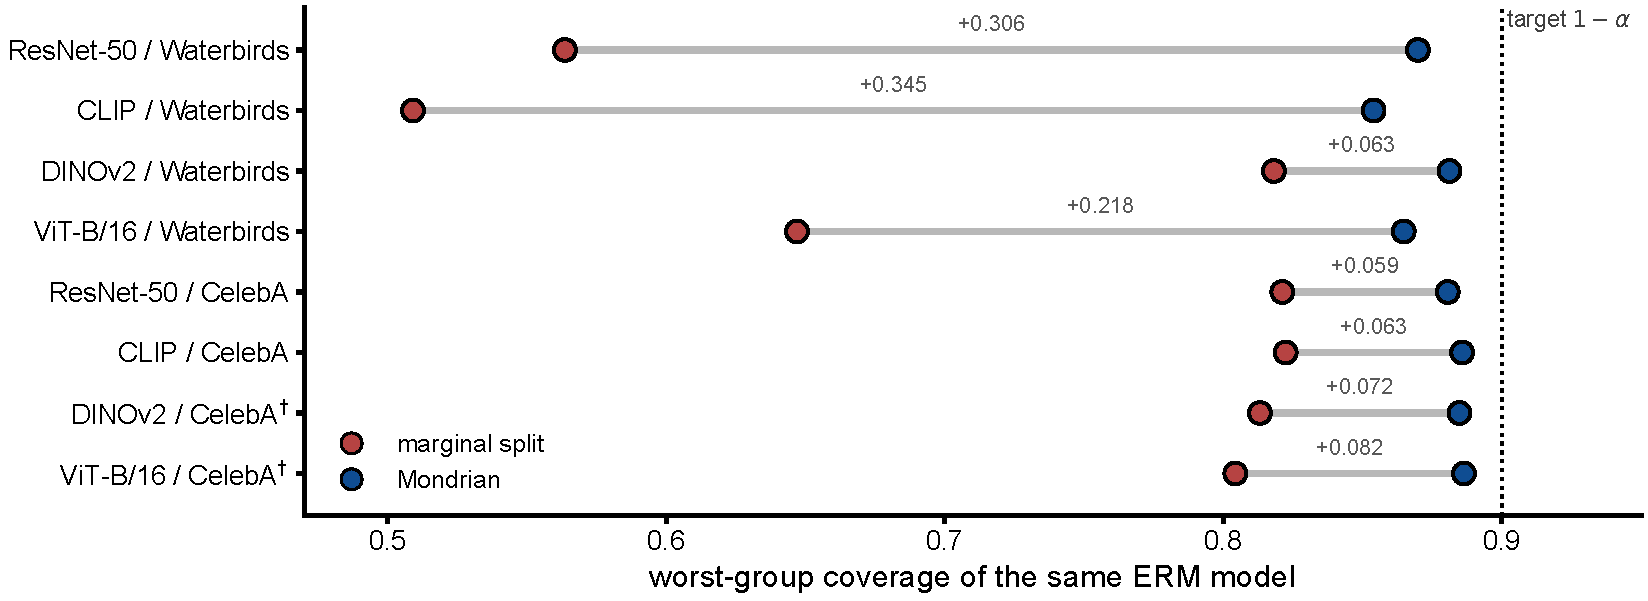
\includegraphics[width=\textwidth]{figures/c1_erm_lift}
\caption{The same ERM model, re-calibrated. Each row is one backbone--dataset cell;
the red point is its worst-group coverage under marginal split and the blue point under
Mondrian, with the lift annotated. Nothing about the model changes between the two
points---only the rule used to turn its scores into sets. The lift is largest exactly
where marginal calibration fails worst, and every Mondrian value lands in
$0.854$--$0.886$ regardless of backbone or dataset. $^{\dagger}$ERM is below its
accuracy floor in these two cells; values are from the sensitivity analysis of
Appendix~\ref{app:excl}.}
\label{fig:c1}
\end{figure}

\begin{table}[t]
\centering
\caption{H\ref{hyp:c1} across all four backbones: worst-group coverage (APS,
$\rhocal=0.95$). The first three columns follow the \emph{same} ERM model under the
two calibration policies; ``spread'' is the range of worst-group coverage across the
retained training arms in that cell. Under marginal calibration the spread reaches
$0.358$ and tracks the training method; under Mondrian it never exceeds $0.024$ in
any of the eight cells. $^{\dagger}$ERM fell below its pre-specified worst-group
accuracy floor in these two cells and is absent from the gate-respecting analysis;
its values here are from the sensitivity run of Appendix~\ref{app:excl} and are
excluded from the spread. Per-method numbers for all three calibration policies, and
for RAPS and THR, are in the released records (Appendix~\ref{app:supp}).}
\label{tab:c1}
\small
\begin{tabular}{lccccc}
\toprule
Backbone / Dataset & ERM marg. & ERM Mond. & ERM lift & spread marg. & spread Mond. \\
\midrule
ResNet-50 / Waterbirds & 0.564 & 0.870 & $+0.306$ & 0.290 & \textbf{0.008} \\
CLIP / Waterbirds & 0.509 & 0.854 & $+0.345$ & 0.358 & \textbf{0.024} \\
DINOv2 / Waterbirds & 0.818 & 0.881 & $+0.063$ & 0.049 & \textbf{0.024} \\
ViT-B/16 / Waterbirds & 0.647 & 0.865 & $+0.218$ & 0.217 & \textbf{0.007} \\
\midrule
ResNet-50 / CelebA & 0.821 & 0.881 & $+0.059$ & 0.071 & \textbf{0.003} \\
CLIP / CelebA & 0.822 & 0.886 & $+0.063$ & 0.059 & \textbf{0.003} \\
DINOv2 / CelebA$^{\dagger}$ & 0.813 & 0.885 & $+0.072$ & 0.013 & \textbf{0.003} \\
ViT-B/16 / CelebA$^{\dagger}$ & 0.804 & 0.886 & $+0.082$ & 0.003 & \textbf{0.008} \\
\botrule
\end{tabular}
\end{table}

\subsection{Moving the Representation Itself}
\label{sec:repr}

Every result so far holds the backbone fixed and varies the last layer, so on its own
it cannot separate ``calibration beats last-layer adaptation'' from ``calibration
beats robust training in general''. This section reports the stronger test: we
fine-tune the backbone \emph{end-to-end} under three objectives---plain ERM,
GroupDRO, and group reweighting---and repeat the comparison on the representations
that result, with five fine-tuning seeds per objective and the head held fixed at
plain ERM so that the representation is the only thing that moves. How much of a
pretrained network to unfreeze is itself consequential, and staged or partial
unfreezing schedules change what a fine-tuned representation encodes
\citep{elmehdi2024unfreezing}; we unfreeze the whole network, so the representation
lever is pulled as far as each objective allows and this is the strongest test of
whether calibration still dominates that our setting admits.

\paragraph{Manipulation check.} A representation-level experiment is informative only
if the intervention actually moved the representation, so we verify that first.
GroupDRO fine-tuning raises worst-group accuracy from $0.516$ to $0.738$ on
Waterbirds ($+0.222$) and from $0.396$ to $0.470$ on CelebA ($+0.074$): the lever was
pulled, and by the largest margin any intervention in this paper produces.
Reweighting did not help ($0.466$ and $0.364$, both slightly below ERM). We report it
regardless---a representation that fails to improve is still a representation that
changed, and dropping it would be selecting on the outcome.

\paragraph{The two levers.} Table~\ref{tab:repr} and Figure~\ref{fig:repr} contrast them. Under marginal
calibration the deployed representation matters: worst-group coverage spans $0.249$
across the three on Waterbirds. Under Mondrian the same three sit within $0.004$ of
one another, all at $\approx\!0.86$, and the ERM representation---the weakest of the
three by worst-group accuracy---is lifted from $0.568$ to $0.865$ by the calibration
switch alone. CelebA repeats the pattern at smaller magnitude ($0.019$ under
marginal, $0.001$ under Mondrian), for the same reason as in
Section~\ref{sec:c1}: its marginal coverage was never as far from target to begin
with.

The dissociation is therefore not an artefact of freezing the backbone. Even when the
representation is genuinely improved, switching the calibration rule buys more
worst-group coverage than switching the representation, and group-conditional
calibration removes almost all of the difference between representations. What the
representation lever does buy is visible in the accuracy column, not the coverage
one---the same efficiency-not-coverage pattern as Section~\ref{sec:c2}.

\begin{figure}[t]
\centering
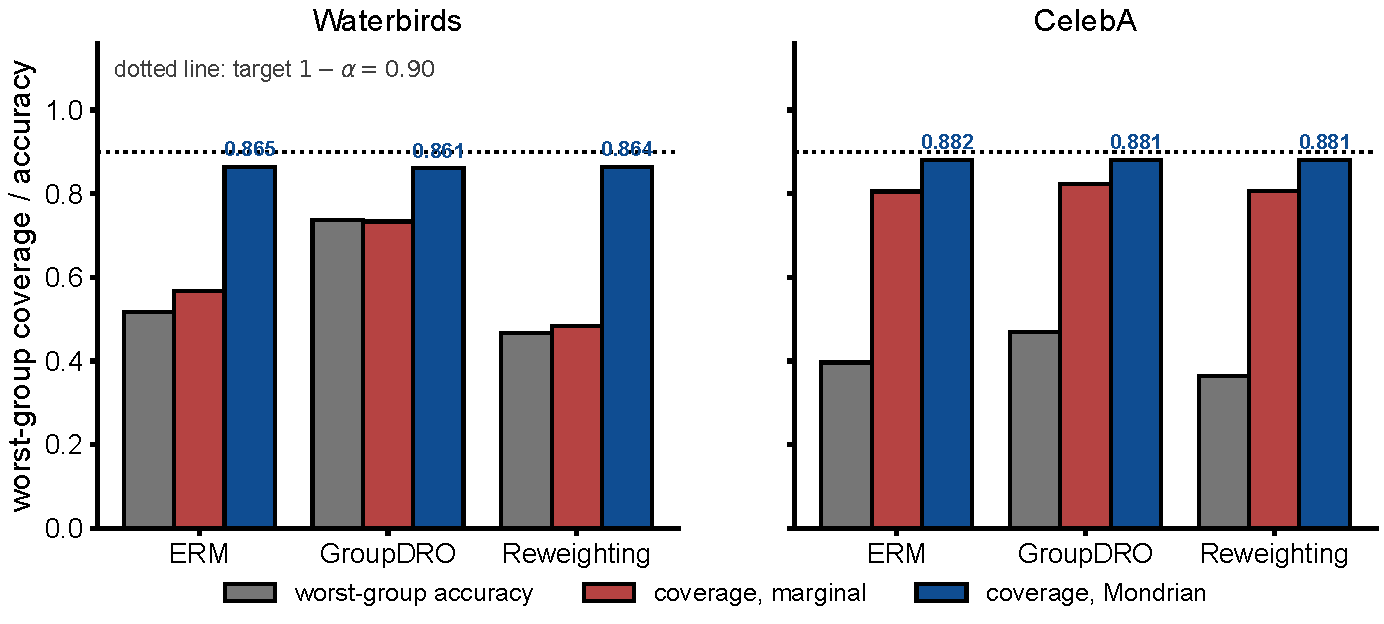
\includegraphics[width=\textwidth]{figures/repr_lever}
\caption{The representation lever, with the head held fixed at plain ERM (APS,
$\rhocal=0.95$, five fine-tuning seeds per objective). Worst-group accuracy (grey) and
worst-group coverage under marginal calibration (red) move together across the three
fine-tuned representations---by $0.222$ and $0.249$ respectively on Waterbirds---while
coverage under Mondrian (blue) does not move at all, spanning $0.004$ on Waterbirds and
$0.001$ on CelebA. Reweighting fine-tuning did not improve the representation and is
reported regardless. Bars begin at zero.}
\label{fig:repr}
\end{figure}

\begin{table}[t]
\centering
\caption{Moving the representation itself. Backbones fine-tuned end-to-end under
three objectives (five seeds each), head held fixed at plain ERM, APS,
$\rhocal=0.95$. GroupDRO fine-tuning improves the representation substantially
(worst-group accuracy $+0.222$ on Waterbirds), yet under Mondrian the three
representations deliver the same worst-group coverage to within $0.004$.}
\label{tab:repr}
\small
\begin{tabular}{llccc}
\toprule
Dataset & Fine-tuned representation & wg acc & marginal & Mondrian \\
\midrule
\multirow{4}{*}{Waterbirds}
 & ERM & 0.516 & \textbf{0.568} & 0.865 \\
 & GroupDRO & \textbf{0.738} & 0.733 & 0.861 \\
 & Reweighting & 0.466 & 0.485 & 0.864 \\
 & \emph{spread} & & \emph{0.249} & \emph{0.004} \\
\midrule
\multirow{4}{*}{CelebA}
 & ERM & 0.396 & 0.805 & 0.882 \\
 & GroupDRO & \textbf{0.470} & 0.824 & 0.881 \\
 & Reweighting & 0.364 & 0.806 & 0.881 \\
 & \emph{spread} & & \emph{0.019} & \emph{0.001} \\
\botrule
\end{tabular}
\end{table}


\subsection{Training Buys Efficiency, Not Coverage (H\ref{hyp:c2})}
\label{sec:c2}

Given that Mondrian equalizes worst-group \emph{coverage} across training methods,
where does training help? Table~\ref{tab:c2} reports worst-group set size under
Mondrian---where coverage is matched---against worst-group accuracy. The direction
agrees with an efficiency reading: in seven of eight cells the most accurate retained
arm also yields the smallest worst-group sets, and ERM yields the largest in every
cell where it is retained.

The per-cell correlation, however, does not survive uncertainty quantification. Each
is computed over the three to five retained methods of that cell, and with a
cluster-bootstrap CI five of the eight span essentially $[-1,+1]$: the $-0.97$ and
$-1.00$ we previously reported on the two original CelebA cells are, at $n=4$, not
evidence of a deterministic relationship. Two cells (CLIP and ViT-B/16 on Waterbirds)
have intervals excluding zero; one (DINOv2/Waterbirds, $+0.22$) points the other way.
We therefore report the accuracy--efficiency link as a \emph{direction} rather than an
estimate, and only under Mondrian: under marginal calibration training still moves
coverage, so ``efficiency, not coverage'' is conditional on the calibration policy
being group-conditional and is not a general statement.

Nor is the spread negligible, as we previously described it. It ranges from $0.036$
(DINOv2/Waterbirds) to $0.364$ (ViT-B/16/Waterbirds), and a two-one-sided-test
equivalence check rejects equivalence at a margin of $0.10$ in six of the eight cells
and at $0.20$ in five. The earlier characterisation of the efficiency range as
``narrow'' was not supported and is withdrawn; what holds is that the differences
appear in efficiency while coverage stays matched.

One number needs disclosure. On DINOv2/Waterbirds the mean worst-group set size is
\emph{below} one ($0.926$--$0.964$ across scores), which means a small fraction of
prediction sets are empty. That is a legitimate outcome of standard split conformal
with a highly accurate model---the calibration quantile can fall below every class
score---and coverage there remains valid under Mondrian ($0.858$--$0.881$). We report
it rather than clipping sets to a minimum size of one, which would hide it.

\begin{table}[t]
\centering
\caption{H\ref{hyp:c2} across all four backbones: worst-group set size under Mondrian
(APS, $\rhocal=0.95$), where coverage is matched across arms. ``best robust'' is the
smallest-set robust arm; ``spread'' is the range across retained arms; ``corr'' is the
Pearson correlation of (worst-group accuracy, worst-group set size) over that cell's
retained methods, with a bootstrap CI. \emph{Italic} CIs span essentially $[-1,+1]$
and are uninformative---five of the eight, because each correlation rests on only
three to five methods. $^{\dagger}$ERM gated out (Appendix~\ref{app:excl}). Set sizes
below $1$ on DINOv2/Waterbirds indicate a small fraction of empty sets, discussed in
the text.}
\label{tab:c2}
\small
\begin{tabular}{lccccc}
\toprule
Backbone / Dataset & ERM & best robust & spread & corr & CI \\
\midrule
ResNet-50 / Waterbirds & 1.138 & 1.101 & 0.116 & $+0.05$ & \emph{$[-1.00,+1.00]$} \\
CLIP / Waterbirds & 1.319 & 1.135 & 0.184 & $-0.85$ & $[-1.00,-0.32]$ \\
DINOv2 / Waterbirds & 0.927 & 0.926 & 0.036 & $+0.22$ & \emph{$[-1.00,+1.00]$} \\
ViT-B/16 / Waterbirds & 1.452 & 1.088 & 0.364 & $-0.91$ & $[-1.00,-0.88]$ \\
\midrule
ResNet-50 / CelebA & 1.378 & 1.091 & 0.287 & $-0.97$ & \emph{$[-1.00,+1.00]$} \\
CLIP / CelebA & 1.163 & 1.041 & 0.122 & $-1.00$ & \emph{$[-1.00,+1.00]$} \\
DINOv2 / CelebA & $^{\dagger}$--- & 1.089 & 0.095 & $-0.70$ & \emph{$[-1.00,+1.00]$} \\
ViT-B/16 / CelebA & $^{\dagger}$--- & 1.105 & 0.039 & $-0.97$ & $[-1.00,-0.97]$ \\
\botrule
\end{tabular}
\end{table}

\subsection{``Transfer'' Is Mostly an Accuracy Effect (H\ref{hyp:h1})}
\label{sec:h1}

The dissociation above predicts that any apparent training-side reduction of the
conformal \emph{burden} should be largely an accuracy effect. Figure~\ref{fig:h1} and
Table~\ref{tab:h1} show the confound directly: ERM's raw APS divergence of $0.14$--$0.22$ falls to
$0.01$--$0.12$ for the robust arms, but base accuracy moves in lockstep, so the raw
number cannot be read as reduced heterogeneity.

Controlling for it turns out to be harder than we previously reported, and the
analysis is re-scoped accordingly. The submitted version pooled each arm's
$(\text{accuracy},D)$ points across seeds \emph{and} calibration splits. That axis is
mostly evaluation-draw noise rather than model variation: ERM's per-seed base accuracy
is identical to five decimals in every cell---its last-layer solver is
deterministic, so the training seed does not move it---and all of its apparent
accuracy spread came from which evaluation rows were drawn. Matching on that spread
compares ERM on unlucky draws against a robust arm on lucky ones, and the
accompanying bootstrap over pooled points treated fifty nested rows as fifty
independent draws.

Recomputed at model level, with one accuracy per training seed and a two-stage cluster
bootstrap that resamples seeds and then splits within them, ERM's accuracy support is a
single \emph{point} and overlapping support exists in exactly one of the eight cells:
GroupDRO-LL on ResNet-50/Waterbirds, whose per-seed accuracies bracket ERM's
$0.9399$. There the reduction is real and replicates the earlier estimate---
$\Delta_{\mathrm{APS}}=+0.084\,[+0.076,+0.095]$,
$\Delta_{\mathrm{RAPS}}=+0.084\,[+0.074,+0.094]$,
$\Delta_{\mathrm{THR}}=+0.150\,[+0.146,+0.158]$, all three CIs excluding zero. The two
further matched values reported in the submitted version (GroupDRO-LL on
CLIP/Waterbirds, balanced subsampling on ResNet-50/Waterbirds) rested on the
split-level spread and are withdrawn: at model level neither arm's accuracy support
reaches ERM's.

We therefore limit H\ref{hyp:h1} to that one matched setting, as the reviewer asks, and
draw no accuracy-matched conclusion elsewhere. The reason the comparison is unavailable
is itself informative and is the more robust reading: on CelebA the robust arms raise
base accuracy to $0.83$--$0.91$ against ERM's $0.68$--$0.70$, so no common operating
point exists at all, and on the remaining Waterbirds cells they trade $4$--$10$ accuracy
points for their robustness. Uncontrolled comparisons of $D$ therefore conflate two
effects across most of the grid, which is exactly the confound this protocol exists to
expose.

\begin{figure}[t]
\centering
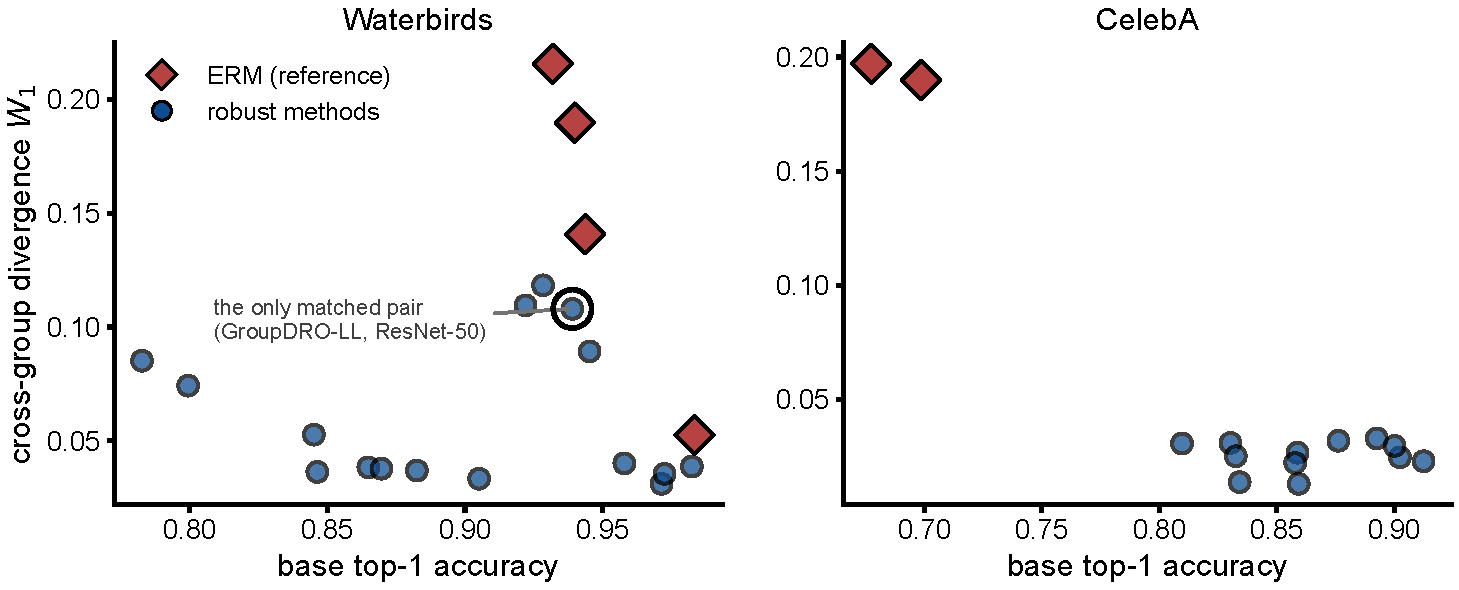
\includegraphics[width=\textwidth]{figures/h1_accuracy_confound}
\caption{Why the accuracy-matched comparison is usually unavailable. Each point is one
arm's mean base accuracy against its cross-group divergence (APS, $\rhocal=0.95$); red
diamonds are the ERM reference of each cell. On CelebA the robust arms occupy
$0.81$--$0.91$ while ERM sits at $0.68$--$0.70$, so no common accuracy exists at which
to compare them. Matching is within a cell, and across the whole grid exactly one
(cell, arm) pair has overlapping per-seed accuracy support---circled.}
\label{fig:h1}
\end{figure}

\begin{table}[t]
\centering
\caption{H\ref{hyp:h1} across all four backbones: the accuracy confound (APS,
$\rhocal=0.95$). The raw cross-group divergence $D$ collapses from ERM to the robust
arms, but base accuracy moves with it, so the raw reduction cannot be attributed to
reduced heterogeneity. The last column names the arms whose \emph{model-level}
accuracy support overlaps ERM's; \texttt{unm.}\ = none does, so $\Delta(a^\star)$ is
undefined. $^{\dagger}$ERM gated out, so no reference exists
(Appendix~\ref{app:excl}). Per-score values for the one matched pair are in the text.}
\label{tab:h1}
\small
\begin{tabular}{lccccc}
\toprule
Backbone / Dataset & $D_{\mathrm{ERM}}$ & acc$_{\mathrm{ERM}}$ & $D$ (robust) & acc (robust) & matched \\
\midrule
ResNet-50 / Waterbirds & 0.190 & 0.940 & 0.038--0.110 & 0.800--0.939 & GroupDRO-LL \\
CLIP / Waterbirds & 0.216 & 0.932 & 0.036--0.118 & 0.783--0.928 & \texttt{unm.} \\
DINOv2 / Waterbirds & 0.053 & 0.983 & 0.031--0.040 & 0.958--0.982 & \texttt{unm.} \\
ViT-B/16 / Waterbirds & 0.141 & 0.944 & 0.033--0.089 & 0.845--0.945 & \texttt{unm.} \\
\midrule
ResNet-50 / CelebA & 0.190 & 0.699 & 0.013--0.031 & 0.810--0.859 & \texttt{unm.} \\
CLIP / CelebA & 0.197 & 0.677 & 0.023--0.030 & 0.900--0.913 & \texttt{unm.} \\
DINOv2 / CelebA$^{\dagger}$ & --- & --- & 0.014--0.032 & 0.830--0.876 & \texttt{no ref.} \\
ViT-B/16 / CelebA$^{\dagger}$ & --- & --- & 0.022--0.033 & 0.833--0.893 & \texttt{no ref.} \\
\botrule
\end{tabular}
\end{table}

\subsection{Worst-Group Accuracy Is a Good Proxy for Conformal Burden (H\ref{hyp:h2})}
\label{sec:h2}

Table~\ref{tab:h2} reports worst-group accuracy and conformal burden $\covgap$ with
the inversion verdict, now with cluster-bootstrap intervals that resample training
seeds and then splits within them. The point-estimate ranking differs between accuracy
and burden in 5 of the eight cells, but the difference is separated from zero in
only 1 of them, and in those it is small in absolute terms. Across the grid the two
rankings are strongly concordant, so worst-group accuracy remains a reasonable---though
not infallible---proxy for worst-group conformal burden. We state it as a tendency
rather than a rule: where the two disagree, the disagreement is within a few
thousandths of coverage and both arms sit near the coverage ceiling.

\begin{table}[t]
\centering
\caption{H\ref{hyp:h2} across all four backbones: the accuracy-best and burden-best
arm per cell (APS, $\rhocal=0.95$), with $\covgap$ and its cluster-bootstrap CI.
``inversion'' is \textbf{real} only when a paired cluster bootstrap of the difference
excludes zero; a parenthesised value is a point-estimate gap whose interval includes
zero, and so is not evidence of an inversion. Point-estimate inversions occur in 5 of
eight cells but survive the interval in 1. Full five-method numbers are in the released
records.}
\label{tab:h2}
\footnotesize
\setlength{\tabcolsep}{3.5pt}
\begin{tabular}{llcclcl}
\toprule
Backbone & acc-best & wg acc & $\covgap$ [CI] & burden-best & $\covgap$ & inversion \\
\midrule
\multicolumn{7}{l}{\emph{Waterbirds}} \\
ResNet-50 & DFR & 0.812 & 0.048\,[0.037,0.060] & DFR & 0.048 & no \\
CLIP & DFR & 0.838 & 0.050\,[0.040,0.062] & Bal.\ sub. & 0.039 & no ($+0.011$) \\
DINOv2 & DFR & 0.949 & 0.036\,[0.030,0.043] & Bal.\ sub. & 0.033 & no ($+0.003$) \\
ViT-B/16 & DFR & 0.877 & 0.035\,[0.028,0.044] & DFR & 0.035 & no \\
\midrule
\multicolumn{7}{l}{\emph{CelebA}} \\
ResNet-50 & DFR & 0.851 & 0.022\,[0.019,0.025] & GroupDRO-LL & 0.008 & \textbf{real} $+0.014$ \\
CLIP & GroupDRO-LL & 0.905 & 0.018\,[0.016,0.020] & GroupDRO-LL & 0.018 & no \\
DINOv2 & GroupDRO-LL & 0.846 & 0.015\,[0.012,0.018] & Bal.\ sub. & 0.014 & no ($+0.001$) \\
ViT-B/16 & GroupDRO-LL & 0.874 & 0.019\,[0.017,0.021] & Bal.\ sub. & 0.018 & no ($+0.001$) \\
\botrule
\end{tabular}
\end{table}

\subsection{Stable but Sub-Target under Shift; No Relocation (H\ref{hyp:h3})}
\label{sec:h3}

\paragraph{What this sweep does and does not vary.} The $\rho$ sweep changes the
\emph{group mixture} of the evaluation distribution---the probability that the
spurious attribute aligns with the label---while the class-conditional feature
distribution within each of the four groups is untouched. It is therefore a
group-prior shift, a special case of label-and-attribute shift, and \emph{not} a
general covariate shift: it does not move the within-group data distribution, corrupt
inputs, or change the domain. Our stability claim is scoped accordingly. It says that
group-conditional calibration is insensitive to how strongly the spurious correlation
is expressed at deployment---the failure mode this literature is concerned with---and
it says nothing about robustness to within-group distribution change, which would need
a different construction and which we do not test.

We sweep $\rhotest$ with calibration fixed at $\rhocal=0.95$
(Figure~\ref{fig:shift}; full tables in Appendix~\ref{app:supp}). Three observations
hold across cells. (i) \emph{Stability}: under Mondrian, worst-group coverage varies
by at most $0.024$ over the whole sweep for every method and cell, and under marginal
split by at most $0.037$. We scope this to those two policies: shift-robust
calibration inflates its level with the observed calibration-to-test distance by
construction, so its coverage rises as $\rhotest$ falls---by up to $0.347$ across the
sweep---which is intended behaviour rather than instability. (ii) \emph{Sub-target}: under Mondrian no
method reaches $0.90$; the stable level is $0.85$--$0.89$, consistent with
group-conditional calibration relocating but not closing the worst-group gap.
Whether this level clears a strict ``$\ge\!0.88$'' validity bar across the sweep is
therefore baseline-dependent: it does on CelebA (level $\approx0.88$) and does not
on Waterbirds (level $\approx0.85$), but the curve is flat in both---this is a
sub-target baseline, not a shift collapse. (iii) \emph{No relocation}: the H1
matched-divergence reduction becomes \texttt{undefined} across the sweep, and
set-size disparity \emph{eases} as $\rho\!\to\!0.5$ in most cells rather than
inflating (only DFR and GroupDRO-LL on CelebA/ResNet-50 show mild growth). The
``relocate, not remove'' phenomenon of \citet{burden2026} is therefore not
observed as a shift effect: the burden simply tracks correlation strength and is
maximal at the calibration point.

The sub-target level is finite-sample, not a failure of the dissociation, and the
evidence for that is a co-scaling. Mondrian's split-to-split standard deviation in
worst-group coverage is $0.023$--$0.034$ on Waterbirds against $0.011$--$0.018$ on
CelebA, and its shortfall from target follows the same ordering---$0.030$--$0.044$
against $0.016$--$0.023$. A shortfall that shrinks with the per-group quantile noise is
the signature of finite-sample worst-group quantile estimation, not of a biased
procedure: the minority groups hold a few percent of each calibration pool, and CelebA's
pools are the larger ones. (An earlier version also claimed Mondrian was $2$--$4\times$
more split-stable than marginal calibration. On the four-backbone data the two are
comparable---marginal's SD is $0.009$--$0.042$---and in two of the eight cells Mondrian
is the less stable of the two, so we withdraw that comparison. Mondrian's advantage here
is in the \emph{level} it attains, not in its variance across splits.)

\begin{figure}[t]
\centering
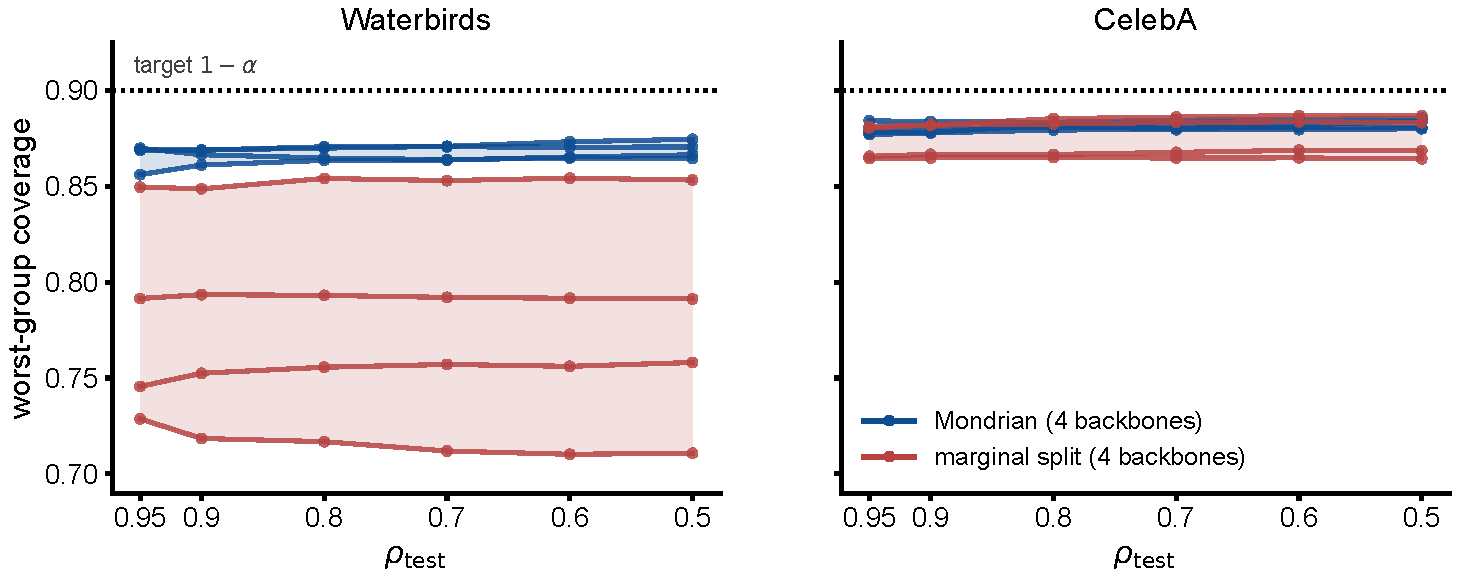
\includegraphics[width=\textwidth]{figures/shift_mondrian_vs_marginal}
\caption{Worst-group coverage against $\rhotest$ with calibration held at
$\rhocal=0.95$, averaged over the retained training arms. One curve per backbone, with
the shaded band the envelope across the four. Blue is Mondrian, red is marginal split.
At the calibration point the Mondrian envelope is $0.014$ wide on Waterbirds and
$0.007$ on CelebA, against $0.121$ and $0.017$ for marginal split: the backbone matters
an order of magnitude less once calibration is group-conditional. Both policies are flat
across the sweep---Mondrian to within $0.010$---and Mondrian sits just below the nominal
$0.90$, which is the min-over-groups effect of Appendix~\ref{app:subtarget} rather than
a shift collapse. The sweep varies the \emph{group mixture} and not the within-group
distribution, so this is stability under group-prior shift, not under general covariate
shift.}
\label{fig:shift}
\end{figure}

\subsection{No Coverage--Auditability Tension (H\ref{hyp:audit})}
\label{sec:audit}

Does the representation on which worst-group coverage is obtained hide the protected
group? It does not. A standardized probe recovers the spurious attribute at
$\auroc\in[0.945,0.999]$ across all eight cells while Mondrian simultaneously
delivers worst-group coverage of $0.854$--$0.886$: coverage and post-hoc group
auditing coexist. Projecting out the top-$k$ spurious-predictive directions
($k\in\{0,1,5,20\}$) leaves coverage flat on ResNet-50 and raises it by at most
$0.02$---still sub-target---as the probe falls toward chance. Forcing invariance does
not unlock coverage; group-conditional calibration already delivers it from a fully
recoverable representation, consistent with H\ref{hyp:c1}.

\subsection{Group-Conditional Calibration Is Deployable with Predicted Groups}
\label{sec:predgroup}

Mondrian uses group labels for per-group thresholds, raising a deployment
objection: are ground-truth groups required? Because the spurious attribute is
highly recoverable (Section~\ref{sec:audit}), they are not---but the mechanics and the
supervision this requires need stating precisely, and so do its limits.

\paragraph{How a predicted attribute sets a threshold.} The label $y$ is never
predicted here; only the spurious attribute is. A probe
$h:\phi(x)\mapsto\hat a\in\{0,1\}$ is fitted on the \emph{training} split's features
and applied to each evaluation point, and the stratum is $\hat g=2y+\hat a$---the true
label with the estimated attribute. Under condition (c), calibration points are binned
by $\hat g$ and each bin's $\lceil(1-\alpha)(n_{\hat g}+1)\rceil$-th smallest score
becomes that bin's threshold $\hat q_{\hat g}$; a test point is assigned to its own
$\hat g$ and admitted to the set if its score is at most $\hat q_{\hat g}$. Coverage is
then tallied against the \emph{true} group, so a mis-assignment is penalised rather
than hidden.

\paragraph{What supervision this needs.} The attribute is required on the training
split, to fit the probe, and nowhere else: not on the calibration split under
condition (c), and never at test time. The label $y$ is still required on the
calibration split, as in any split-conformal method. So the reduction is from
``attribute labels on calibration \emph{and} test data'' to ``attribute labels on
training data only''---a meaningful weakening of the requirement, not its removal.

\paragraph{How probe error propagates.} A mis-assigned point is calibrated against
another group's threshold. The direction matters: the minority stratum carries the
\emph{largest} threshold, so a minority point mistakenly placed in a majority stratum
is judged against a tighter threshold and is under-covered, while the reverse error
merely wastes efficiency. Worst-group coverage therefore degrades asymmetrically with
probe error: over-covering a majority stratum costs efficiency, under-covering the
minority costs validity.

The mechanism is sound but its magnitude is \emph{not} ordered by probe accuracy, and
we were careful to check rather than assume. Across our eight cells the probe's
$\auroc$ does not predict which arms fail: the cell with the \emph{lowest} $\auroc$
($0.945$, ResNet-50/Waterbirds) has no failures at all, while a cell with $\auroc=0.999$
(CLIP/CelebA) has one. What does travel with the penalty is the arm: the two largest
failures are ERM, whose minority points sit closest to the decision boundary and are
the ones a probe most often misplaces. So the probe's $\auroc$ is necessary to report
alongside any coverage claim that relies on it, but it is not sufficient---the arm's own
group-dependence matters as much.

We re-run Mondrian with probe-predicted groups in three conditions: (a) true groups;
(b) predicted groups at test only (thresholds from true-group calibration); and (c)
predicted groups at \emph{both} calibration and test---the fully deployable setting in
which the attribute is never observed outside training. Coverage is always scored on
the true groups.

Table~\ref{tab:predgroup} reports the deployable setting (c) against the oracle (a)
for APS. The penalty is small and it is concentrated where the mechanism above predicts.
Across all eight cells the probe reaches $\auroc\in[0.945,0.999]$, the median
$|\cov(a)-\cov(c)|$ per cell is $0.001$--$0.013$, and 30 of 34 arms clear a
$0.02$ bar. The four failures are ERM on CLIP/Waterbirds ($0.051$) and on
DINOv2/Waterbirds ($0.024$), AFR on ViT-B/16/Waterbirds ($0.022$), and GroupDRO-LL on
CLIP/CelebA ($0.025$). Three of the four are on Waterbirds, whose evaluation pool is
five times smaller, and three of the four exceed the bar only marginally; the one
substantial penalty is ERM on CLIP/Waterbirds, a model one would not deploy for
worst-group reliability in the first place. Probe accuracy does not order them---the
lowest-$\auroc$ cell has no failures and a cell at $\auroc=0.999$ has one---so we
attribute the penalty to the arm's group-dependence rather than to probe error alone. THR is the least stable score
under predicted groups and APS and RAPS behave alike (Appendix~\ref{app:supp}). This closes the loop with H\ref{hyp:audit}: the \emph{same}
recoverability that makes the representation auditable also makes group-conditional
calibration deployable without observed group labels.

\paragraph{What inferring the attribute means, and when it is not acceptable.} This
variant works by predicting a protected attribute for individuals, and that deserves
more than a disclaimer. Two points come first. CelebA's \texttt{Male} field is a
binary annotation applied by third parties to photographs; it is not self-identified
gender, and a study that treats it as gender has erred before any ethical question
arises. We use it because it is the benchmark's standard spurious attribute and
because our claim is about \emph{calibration strata}, not about people---but the
stratum it induces should be read as ``the annotation that co-varies with hair colour
in this dataset'', nothing more. Second, inferring such an attribute at test time is a
materially different act from conditioning on one a person has disclosed: it assigns a
sensitive label to someone who has not provided it, and the assignment is wrong for
$2$--$5\%$ of people even at the $\auroc$ we measure.

We therefore scope the recommendation rather than making it generally. Predicted-group
Mondrian is appropriate where the attribute is already lawfully held or where the
inference stays inside an audit the operator runs on their own system---measuring
whether their own deployed model under-covers a subpopulation, without the inferred
label leaving that audit or reaching any per-person decision. It is not appropriate
where the inferred attribute would be stored, disclosed, or used to route individual
outcomes; in those settings the true-group variant (condition~(a) or~(b)) should be
used with attributes obtained by consent, and where no attribute is available at all,
group-conditional calibration is simply not the right tool. Regulatory regimes that
restrict processing of special-category data may prohibit the inference outright
regardless of accuracy. We report the deployable variant because the objection it
answers---``Mondrian needs group labels you will not have''---is a real one, not
because inferring protected attributes is a neutral default.

\begin{table}[t]
\centering
\caption{Deployable Mondrian across all four backbones (APS,
$\rhocal{=}\rhotest{=}0.95$): the cost of replacing ground-truth groups with
probe-predicted ones at both calibration and test. ``gap'' is
$|\cov(a)-\cov(c)|$ over the cell's retained arms; ``deploy.'' counts those within
$0.02$; the last column names the arm responsible for the maximum where a cell has any
failure. Per-arm values for all three conditions and all three scores are in the
released records.}
\label{tab:predgroup}
\footnotesize
\setlength{\tabcolsep}{3.5pt}
\begin{tabular}{lccccl}
\toprule
 & & \multicolumn{2}{c}{gap} & & \\
\cmidrule(lr){3-4}
Backbone & probe $\auroc$ & median & max & deploy. & worst arm \\
\midrule
\multicolumn{6}{l}{\emph{Waterbirds}} \\
ResNet-50 & 0.945 & 0.007 & 0.012 & 5/5 & --- \\
CLIP & 0.976 & 0.008 & 0.051 & 4/5 & ERM \\
DINOv2 & 0.961 & 0.010 & 0.024 & 4/5 & ERM \\
ViT-B/16 & 0.964 & 0.006 & 0.022 & 4/5 & AFR \\
\midrule
\multicolumn{6}{l}{\emph{CelebA}} \\
ResNet-50 & 0.962 & 0.003 & 0.005 & 4/4 & --- \\
CLIP & 0.999 & 0.011 & 0.025 & 3/4 & GroupDRO-LL \\
DINOv2 & 0.999 & 0.012 & 0.013 & 3/3 & --- \\
ViT-B/16 & 0.993 & 0.001 & 0.003 & 3/3 & --- \\
\botrule
\end{tabular}
\end{table}

\section{Discussion}
\label{sec:discussion}

The results compose into a single thesis. Worst-group \emph{coverage} is governed
chiefly by the calibration policy: marginal calibration leaves it at the mercy of the
representation (ERM collapses), while Mondrian makes it nearly invariant to training
and lifts even ERM to match a robustly trained model (H\ref{hyp:c1}). That holds when
the representation itself is retrained, not only when a new head is fitted on frozen
features (Section~\ref{sec:repr}); training instead buys \emph{efficiency}, and only
once calibration is group-conditional (H\ref{hyp:c2}). Everything else follows: the
apparent training-side reduction of conformal burden is largely an accuracy effect,
and at matched model-level accuracy it is measurable in only one of eight cells
(H\ref{hyp:h1}); accuracy-best is almost always burden-best (H\ref{hyp:h2}); under
correlation-strength shift coverage is stable, and sub-target only in the
min-over-groups sense (H\ref{hyp:h3}); and the representation does not hide the group,
so coverage and auditability coexist (Section~\ref{sec:audit}). The dominant lever is
the calibration \emph{mechanism} rather than the score \emph{representation}---not the
only one, but by a wide margin.

The recommendation is deflationary and useful: (a) report
conformal-burden comparisons \emph{at matched accuracy}, since uncontrolled
comparisons overstate training-side benefits by an order of magnitude; (b) do not
expect a training method chosen for worst-group accuracy to be suboptimal for
conformal burden; and (c) obtain worst-group coverage from group-conditional
calibration, which remains effective on ordinary, fully auditable representations
and---because the group is recoverable---is deployable with probe-predicted groups
(Section~\ref{sec:predgroup}), so test-time group labels are not required.

\section{Limitations}
\label{sec:limitations}

Our conclusions are empirical and scoped to two vision benchmarks, four frozen
backbones plus one fine-tuned end-to-end, and binary spurious attributes; a third
dataset and a multi-class task would extend breadth, though the consistency of
H\ref{hyp:c1} across all eight frozen cells and all six cells of the fine-tuning study
suggests additional data would refine rather than overturn it. The fine-tuning study
moves the representation for one architecture only, so its evidence is narrower than
the frozen grid's. The accuracy-matched comparison
(H\ref{hyp:h1}) is undefined when a method's accuracy support does not overlap
ERM's, which is itself informative but prevents a uniform statement. Because
$|\mathcal{Y}|=2$, set sizes lie in $[1,2]$, compressing the efficiency axis
(H\ref{hyp:c2}); multi-class tasks would give it more range. Mondrian's
group-conditional coverage is, by construction, close to a per-group target, so
H\ref{hyp:c1}'s non-trivial content is the \emph{magnitude} of marginal
calibration's representation-dependent failure and the size of the ERM lift, which
we quantify. Deployable Mondrian (Section~\ref{sec:predgroup})
holds for APS/RAPS and robust arms but degrades for the most group-dependent
model and the THR score, scoping that claim to robust models and rank-based scores;
it also infers a protected attribute at test time, so it should be used only where
such inference is permissible and auditable. Confidence intervals do not model
cross-dataset variance.

\section{Conclusion}
\label{sec:conclusion}

Across a confound-controlled grid, the honest answers are: worst-group coverage
is governed far more by the calibration policy than by the representation---even when
the representation is retrained end-to-end; training buys efficiency rather than
coverage, and only once calibration is group-conditional; the conformal ``transfer''
is mostly an accuracy effect, and at matched model-level accuracy it is measurable in
only one of eight cells; the accuracy--burden inversion is rare; coverage is stable
under correlation-strength shift and sub-target only in the min-over-groups sense; and
there is no auditability tension. We release the full $4\times2\times5\times3\times3$
grid, the representation-level study, the shift sweep, and the accuracy-matched
protocol so that future training-side conformal claims can be evaluated without the
accuracy confound.


\backmatter
\bmhead{Data and code availability}
Waterbirds and CelebA are public. All experiment records, the calibration ablation,
predicted-group results, per-aggregate variance, the quality-gate log, and figure
scripts are released: \texttt{grid\_records.csv} ($36{,}000$ records),
\texttt{calibration\_ablation\_4bb.csv} ($64{,}800$),
\texttt{predicted\_group\_mondrian\_4bb.csv} ($10{,}800$),
\texttt{representation\_records.csv} ($4{,}320$), together with the quality-gate log and
all figure scripts. The conformal layer re-runs in minutes on cached scores without GPU
retraining.

\section*{Declarations}
\textbf{Funding.} The authors received no specific funding for this work.
\textbf{Competing interests.} The authors have no competing interests relevant to
this article. \textbf{Ethics approval.} Not applicable; this study uses only public
benchmark datasets and involves no human participants or animals. \textbf{Data and
code availability.} See ``Data and code availability'' above. \textbf{Author
contributions.} O.O.\ designed and ran the experiments and wrote the manuscript;
N.Y.\ and Y.N.\ supervised the work and revised the manuscript. All authors approved
the final version.

\begin{appendices}
\section{Supplementary Results and Released Records}
\label{app:supp}

All per-(cell, score, method) numbers behind the main tables are in the released
records; this appendix states what each file contains and the few qualitative
summaries that do not fit the main text.

\textbf{Calibration ablation} (\texttt{calibration\_ablation\_4bb.csv}, $64{,}800$
records). Worst-group and mean-over-group coverage, coverage gap, set size and
set-size disparity for every (backbone, dataset, method, seed, split, score,
$\rhotest$, calibration policy), with the gate status of each arm. The dissociation of
Section~\ref{sec:c1} holds for RAPS and THR as well as APS, THR with slightly larger
residual variance. The \emph{shift-robust} policy over-covers the worst group
($0.84$--$0.96$) at the cost of larger sets and is most useful when $\rhotest$ is
expected to move far from $\rhocal$; like Mondrian, it makes worst-group coverage far
less training-dependent than marginal calibration.

\textbf{Grid records} (\texttt{grid\_records.csv}, $36{,}000$ records). Adds the
cross-group divergences and base accuracy per arm, over five training seeds. Under the
$\rhotest$ sweep the set-size disparity \emph{eases} or is flat in every cell except
DFR and GroupDRO-LL on CelebA/ResNet-50, and worst-group coverage has range $<0.05$
and is sub-target for every method---the numbers behind Section~\ref{sec:h3}.

\textbf{Representation study} (\texttt{representation\_records.csv}). The fine-tuning
arms of Section~\ref{sec:repr}: three objectives $\times$ five seeds $\times$ three
heads $\times$ two datasets $\times$ three scores, under marginal and Mondrian
calibration.

\textbf{Predicted-group Mondrian}
(\texttt{predicted\_group\_mondrian\_4bb.csv}). All three conditions (true /
predicted-at-test / predicted-at-both) for every arm. APS and RAPS behave alike; THR
is the least stable score under predicted groups, as small perturbations of the top-$1$
softmax mass matter more when a stratum is mis-assigned, so we scope the
deployable-Mondrian claim of Section~\ref{sec:predgroup} to APS and RAPS.

\section{Why Mondrian Sits Below Target: The Min-over-Groups Effect}
\label{app:subtarget}

Mondrian's empirical worst-group coverage settles at $0.85$--$0.89$ rather than the
nominal $0.90$ (Section~\ref{sec:c1}). This appendix shows the level is what an
\emph{exactly valid} procedure produces at our calibration sizes, so it is a property
of the reported statistic and not a validity failure.

Two effects combine, both finite-sample. First, per-group split conformal with the
finite-sample-corrected quantile
$\lceil(n_g+1)(1-\alpha)\rceil$ covers at $\ge1-\alpha$ \emph{in expectation over
calibration draws}, but we report $\min_g\cov_g$, and the minimum of
$|\mathcal{G}|$ noisy coverages is biased low: for approximately Gaussian per-group
coverages with standard deviation $\sigma$, $\mathbb{E}[\min_g\cov_g]\approx
(1-\alpha)-c_{|\mathcal{G}|}\sigma$ with $c_4\approx1.03$. Second, Mondrian estimates
each threshold from that group's \emph{own} calibration sample, and at $\rhocal=0.95$
the two minority groups hold only $2.5\%$ of the pool each---a $19\times$ imbalance in
threshold precision relative to the majority groups.

Figure~\ref{fig:subtarget} puts our own runs against that law directly, and
Table~\ref{tab:subtarget} simulates the same effect with no model, no data and no
representation: four groups, i.i.d.\ continuous scores, exact exchangeability, per-group
conformal thresholds, and only the realised per-group calibration counts varied.

\begin{figure}[t]
\centering
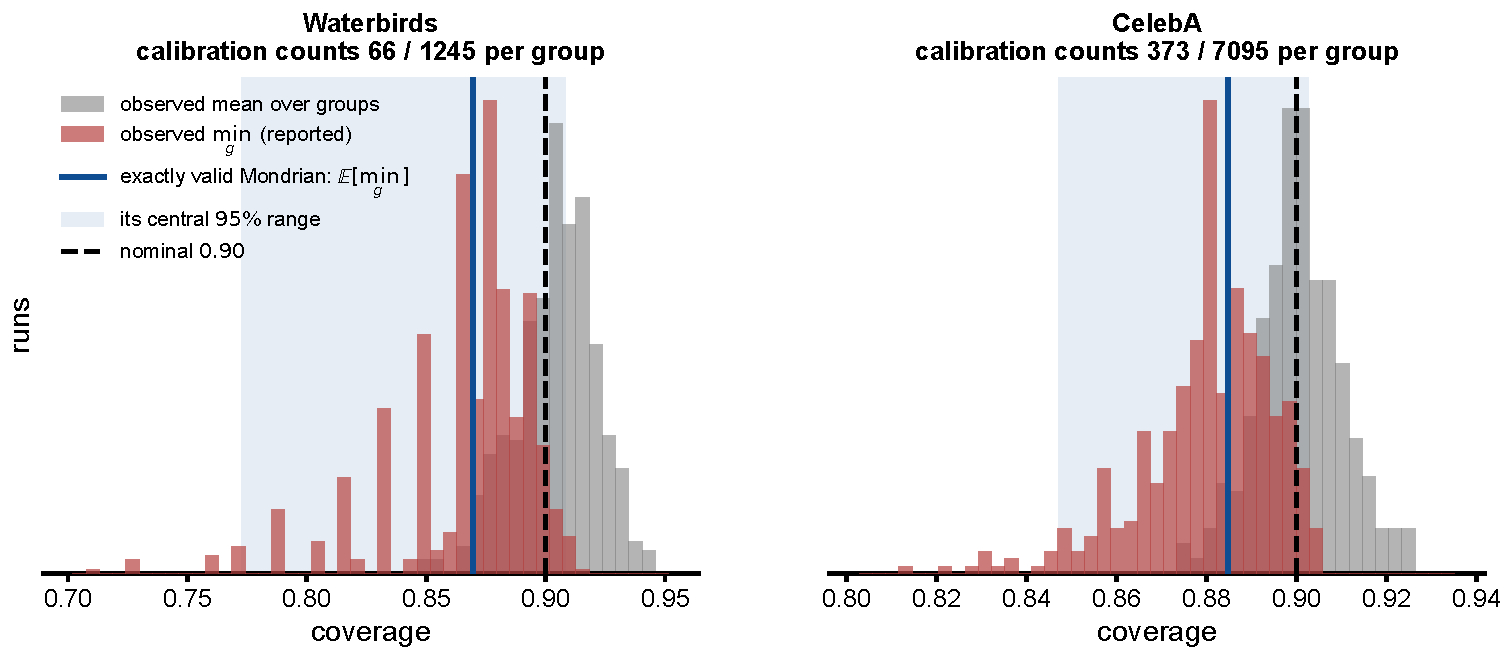
\includegraphics[width=\textwidth]{figures/subtarget_law_vs_observed}
\caption{The sub-target level is a property of the statistic, not evidence of
under-coverage. Each panel pools every retained Mondrian run of that dataset (APS,
$\rhocal=\rhotest=0.95$; $600$ and $410$ runs). The unweighted mean over groups
(grey)---what group-conditional calibration targets---is centred on the nominal $0.90$,
while the \emph{minimum} over four noisy per-group coverages (red), the number we
report, sits below it. The blue line is where an \emph{exactly valid} Mondrian
procedure puts that minimum, simulated at our own per-group calibration and test
counts with no model and no data ($8000$ draws): $0.8695$ against an observed
$0.8660$ on Waterbirds and $0.8847$ against $0.8800$ on CelebA, with $98\%$ and $95\%$
of runs inside its
central $95\%$ range. The observed spread is wider than that range by construction,
since the simulation varies only the calibration and test draw while the runs also vary
over backbones, training arms and seeds; the agreement to be read here is in location.
The effect is larger on Waterbirds, whose minority calibration counts are $66$ against
CelebA's $373$.}
\label{fig:subtarget}
\end{figure}

\begin{table}[t]
\centering
\caption{Worst-group coverage of an \emph{exactly valid} Mondrian procedure under pure
exchangeability, by calibration-pool size at $\rhocal=0.95$ (groups ordered $2y+a$;
$\alpha=0.10$; $3000$ draws). The mean over groups sits at the nominal $0.90$ while the
\emph{minimum} does not: the shortfall is the min-over-groups selection effect, and it
shrinks as the minority calibration counts grow.}
\label{tab:subtarget}
\small
\begin{tabular}{rlccc}
\toprule
cal.\ pool & per-group counts & mean over groups & $\mathbb{E}[\min_g\cov_g]$ & shortfall \\
\midrule
$500$    & $238/13/13/238$      & 0.915 & 0.842 & 0.058 \\
$1{,}000$  & $475/25/25/475$      & 0.913 & 0.858 & 0.042 \\
$2{,}000$  & $950/50/50/950$      & 0.901 & 0.856 & 0.044 \\
$5{,}000$  & $2375/125/125/2375$  & 0.902 & 0.874 & 0.026 \\
$10{,}000$ & $4750/250/250/4750$  & 0.900 & 0.880 & 0.020 \\
\botrule
\end{tabular}
\end{table}

The simulated shortfalls, $0.02$--$0.06$, bracket the $0.016$--$0.044$ we observe, and the
observed values track calibration size in the same direction---larger on Waterbirds,
smaller on the much larger CelebA pools. The diagnostic that settles it is the
unweighted mean over groups, which is the level group-conditional calibration actually
targets: across our eight Mondrian cells it is $0.9024$ (range
$0.8995$--$0.9056$) against a nominal $0.90$, while the mean of the per-cell
\emph{minima} is $0.8728$. The $0.0295$ between them is the selection
effect of reporting a minimum, not under-coverage. We continue to report
$\min_g\cov_g$ because it is the operationally relevant number, but we report the mean
over groups alongside it so the two are not confused.

\section{Excluded and Flagged Arms, and Their Influence}
\label{app:excl}

\paragraph{Status of the rules.} The per-method worst-group accuracy floors were fixed
in the codebase on 11 June 2026, three months before any run reported here, so they
are \emph{pre-specified} with respect to every number in this paper. They were not
lodged in a public registry, so they are not \emph{preregistered}, and we do not claim
to be. The floors are $0.30$ for ERM and $0.75$ for the robust arms on CelebA, and
$0.30$/$0.40$--$0.45$ on Waterbirds.

\paragraph{What was excluded.} $33$ of $200$ arms: AFR on all four CelebA backbones,
all seeds ($0.013$--$0.434$); ERM on DINOv2/CelebA ($0.203$) and ViT-B/16/CelebA
($0.263$); GroupDRO-LL seeds $1$ and $4$ on CelebA/ResNet-50 ($0.676$, $0.683$); and
balanced subsampling seed $4$ there ($0.730$). Twelve DFR arms on CelebA sit just below
a soft reference of $0.85$ ($0.808$--$0.847$) and are kept, flagged.

\paragraph{AFR's collapse is not an untuned hyperparameter.} AFR reaches
$0.686$--$0.890$ worst-group accuracy on Waterbirds but $0.013$--$0.029$ on the three
ViT backbones of CelebA. The mechanism is a class-prior inversion: at the default
$\gamma=2$ the reweighting drives the head to predict the positive class for
$\approx\!86\%$ of examples where the true rate is $\approx\!15\%$, so a
\emph{majority} group becomes the worst group. It is monotone in $\gamma$, and
$\gamma=1$ improves on ERM. Because reporting a method at an untuned hyperparameter
would be unfair, we computed an \emph{oracle} upper bound---the best $\gamma$ chosen
with knowledge of the evaluation set, which no selection rule could beat: $0.327$,
$0.427$, $0.445$ and $0.477$ across the four CelebA backbones, all far below the
$0.75$ floor. AFR's exclusion is therefore a property of the method in this regime,
not of our choice of $\gamma$.

\paragraph{Influence of the excluded arms (R2.4).} We recomputed every verdict with
the gated arms included. The dissociation is unaffected: under Mondrian the
across-training spread rises only to $0.028$ at worst, against $0.024$ with the arms
excluded, while the marginal spread grows because the degenerate arms are themselves
badly under-covered. One thing does change and we report it: the pre-specified C1
criterion---Mondrian within $0.02$ of target \emph{and} marginal significantly below
target for \emph{every} method---is met in exactly one of eight cells (CLIP/CelebA),
and that single cell \emph{flips} to failing when the gated AFR arm is included, since
AFR's marginal coverage there is $0.695$. The criterion is thus not robust to the gate
decision, and we rest the claim on the spread magnitudes rather than on the
pass/fail flag. Including a degenerate arm also produces a spurious H\ref{hyp:h1}
signal for AFR on CelebA/ResNet-50, which is a further reason to report both readings
rather than either alone.

\section{Procedures, Hyperparameters, and Statistics}
\label{app:hyper}
\textbf{Features.} Frozen ERM ResNet-50 ($d{=}2048$) and CLIP ViT-B/32 ($d{=}512$),
extracted once and cached; all training is last-layer on cached features.
\textbf{Heads.} ERM (cross-entropy); DFR (group-balanced last-layer retraining);
AFR (automatic feature reweighting); balanced subsampling; last-layer GroupDRO.
\textbf{Calibration.} marginal split (one global quantile); Mondrian (a separate
quantile per group $g$, with a fallback to the pooled quantile when a group's
calibration count $n_g<50$); shift-robust (worst-case threshold over a
total-variation ball of radius $\epsilon=0.1$ around the calibration distribution;
results are insensitive over $\epsilon\in[0.05,0.2]$, trading $1$--$5$ points of
over-coverage for stability); $1-\alpha=0.90$. \textbf{Scores.} THR, APS, RAPS
(with standard tail regularization). \textbf{Shift.}
$\rhocal=0.95$; $\rhotest\in\{0.95,0.9,0.8,0.7,0.6,0.5\}$ via reweighted/composited
evaluation distributions, with realized $\rho$ logged. \textbf{Seeds/splits.}
$\ge3$ training seeds $\times\ge10$ calibration splits; $95\%$ CIs by bootstrap;
training-seed standard deviation and calibration-split standard deviation reported
separately per aggregate. \textbf{Accuracy matching.} accuracy is overall (base)
top-1 on the evaluation distribution; from the per-seed $(\mathrm{acc},D)$ clouds of
$m$ and ERM we take $a^\star$ in the overlapping accuracy range and read each
method's $D(a^\star)$ by linear interpolation of its cloud, bootstrapping over
seeds; $\Delta(a^\star)$ is \texttt{unmatched} when the supports are disjoint.
\textbf{Recoverability.} StandardScaler $\to$ logistic
regression, in-domain train$\to$test; invariant-ization by projecting out the
top-$k$ spurious-predictive directions, $k\in\{0,1,5,20\}$. \textbf{Predicted-group
Mondrian.} the recoverability probe predicts the stratum $2y+\hat a$; thresholds
and/or test assignment use $\hat a$; coverage is always scored on true groups.
\textbf{Calibration/test construction (exact).} For each of $10$ split seeds the
evaluation pool is partitioned once into disjoint halves by a seeded permutation; the
first half is the calibration reservoir and the second the test reservoir, so no row is
ever in both. Each reservoir is then resampled to its target correlation
strength---$\rhocal=0.95$ for calibration, $\rhotest$ for test---by drawing within that
reservoir's own group indices, and both draws are truncated to a common size
$n=\min(|\mathrm{cal}|,|\mathrm{test}|)$ so calibration and test sizes never differ
across $\rho$. The realised $\rho$ is logged per draw. Randomised scores (APS, RAPS)
take their tie-breaking uniforms from separate seeded streams for calibration and test.
\textbf{Per-group counts.} Waterbirds: train $4{,}795$, evaluation pool $5{,}245$, with
the reweighting split holding $663/706/202/177$ for groups $2y+a=0,1,2,3$. CelebA: train
$162{,}770$, evaluation pool $29{,}872$, reweighting split $4{,}650/3{,}895/1{,}331/81$.
Under Mondrian the worst group's calibration count never falls below $50$ in any cell:
its minimum is $66$ on Waterbirds and $373$ on CelebA, so the pooled-quantile fallback
is never triggered by the runs reported here.
\textbf{Head hyperparameters.} Every head standardises features using train-split
statistics, then fits a multinomial logistic model with L-BFGS, $C=1$ and at most
$5000$ iterations. DFR averages $10$ group-balanced subsamples; balanced subsampling
draws one; AFR uses $\gamma=2$, whose sensitivity is examined in
Appendix~\ref{app:excl}; last-layer GroupDRO runs $2000$ full-batch steps at learning
rate $0.05$ with group-weight step $\eta_q=0.05$ and $\ell_2$ penalty $10^{-3}$.
Fine-tuning (Section~\ref{sec:repr}) starts from ImageNet-V2 weights and uses Adam at
$10^{-3}$ for ERM and reweighting, SGD at $10^{-3}$ with weight decay $10^{-2}$ for
GroupDRO, batch size $128$, mixed precision, and the last epoch rather than a selected
one.
\textbf{Shift-robust procedure (exact).} Given the calibration scores and the observed
total-variation distance $\epsilon$ between the calibration and test true-label score
distributions, the threshold is the $\min(1,\,(1-\alpha)+\epsilon)$ empirical quantile of
the calibration scores---the smallest level that guarantees $1-\alpha$ coverage for any
reweighting inside the TV ball.
\textbf{Seeds.} Training seeds $\{0,1,2,3,4\}$ for the grid and the fine-tuning study,
$\{0,1,2\}$ for the calibration and predicted-group ablations; calibration split seeds
$0$--$9$ throughout; bootstrap seeds fixed at $0$. Note that ERM and AFR are
deterministic given the cached features, so their across-seed variance is exactly zero.
\textbf{Compute.} The full grid and both ablations re-calibrate cached head posteriors,
and feature extraction runs once per backbone. The four-backbone grid takes $200$
minutes, the calibration ablation $183$, and the predicted-group study $92$, all on a
single machine with no GPU retraining.
\textbf{Archival code.} \emph{[To be replaced before publication with the archived DOI of
the tagged release.]} The archive contains the module that produces each table, the
notebooks that generated the records, and the exact commands needed to reproduce every
released CSV from the cached features. \textbf{Release.} \texttt{grid\_records.csv},
\texttt{calibration\_ablation\_4bb.csv}, \texttt{predicted\_group\_mondrian\_4bb.csv},
\texttt{representation\_records.csv}, per-aggregate JSON (seed-std vs split-std), the
quality-gate log, and all figure scripts are released.

\end{appendices}

\bibliography{sn-bibliography}

\end{document}